\chapter{Multiscale Models for Pebble Bed Reactors}
\label{sec:PhysicalModels}

Many man-made and natural systems exhibit wide ranges in temporal and/or spatial scales such that the use of models applicable to the ``smallest common denominator'' scale for all length scales are computationally impractical. Examples of such systems include Earth's climate, drugs targeting cancer cell growth, and \glspl{pbr}. Multiscale analysis is based on decomposing a complex system into a number of important temporal and spatial length scales, each described by different models, that are aggregated together in an intelligent manner to obtain a representative solution for the relevant physical phenomena on all length scales. The underlying motivation is to enable comprehensive physics predictions at significantly reduced computational cost relative to fine-scale modeling of all scales. 

\glspl{pbr} are naturally described in terms of three length scales\mdash 1)~the macroscale, defined over the entire reactor core, which encompasses the pebble bed, reflectors, and structural materials; 2)~the mesoscale, defined over a single pebble; and 3)~the microscale, defined over a single fuel particle. Fig.\ \ref{fig:multiscale} depicts these three length scales for the pebble bed region. For a typical \gls{pbr}, the characteristic macro, meso, and micro length scales are approximately \(5\times10^0\) m, \(5\times10^{-2}\) m, and \(1\times10^{-3}\) m, respectively, such that the mesoscale is approximately 100 times smaller than the macroscale and the microscale is approximately 50 times smaller than the mesoscale. 

\begin{figure}[!h]
\centering
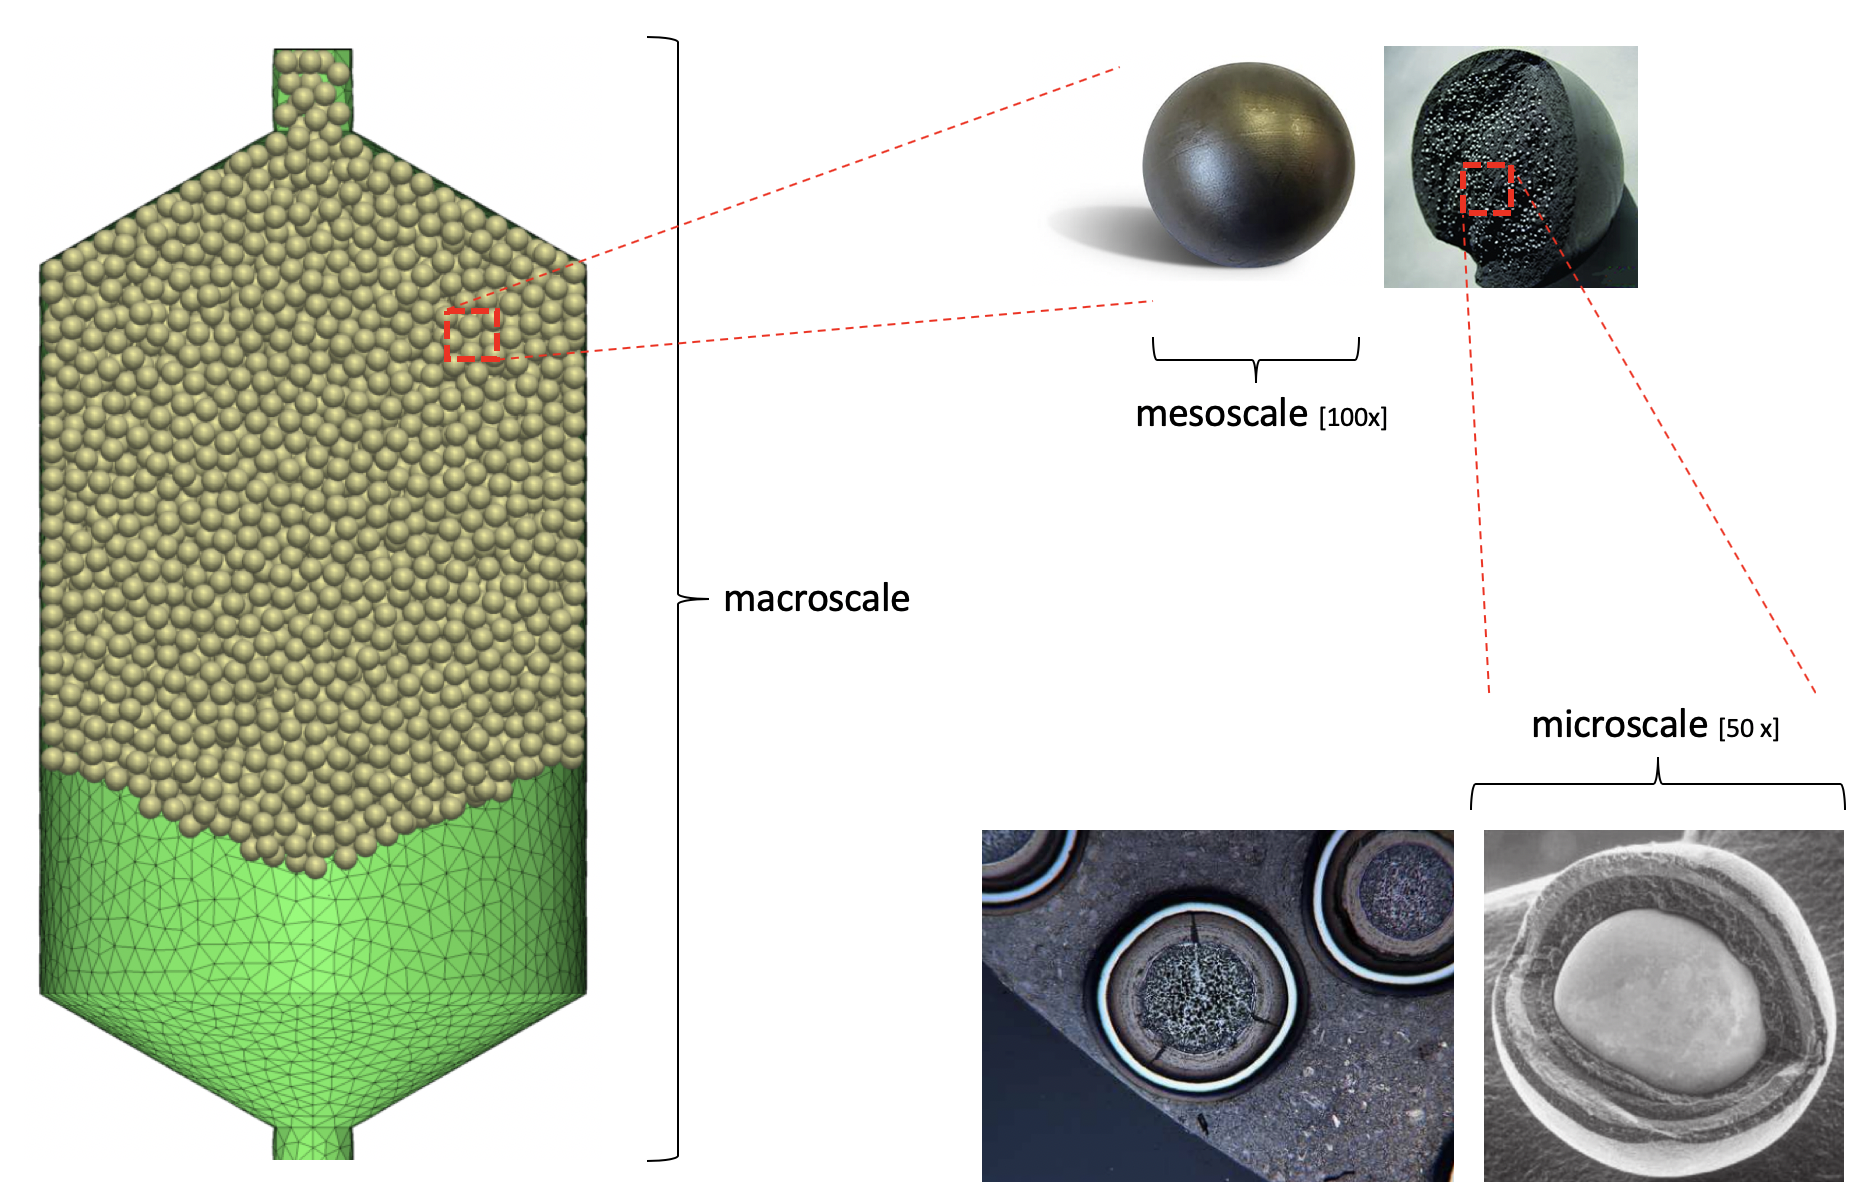
\includegraphics[width=\linewidth]{figs/multiscale_pbr.png}
\caption{Decomposition of a \gls{pbr} into three length scales (adapted from \cite{aufiero_2016,pebble_cut,pebble_uncut,triso_closeup,hales}).}
\label{fig:multiscale}
\end{figure}

By assuming fine length scales are periodic with respect to coarse length scales, \glspl{bc} from the coarser-length solution are applied to finer-scale models to obtain representative thermal and flow predictions for all length scales. This section describes the multiscale modeling approach developed in this dissertation in terms of the three length scales shown in Fig.\ \ref{fig:multiscale}. Section \ref{sec:macro_deriv} discusses the macroscale model, while Section \ref{sec:mesomicro} discusses the mesoscale and microscale models. Finally, Section \ref{sec:MacroAssumptions} elaborates on the most important limitations, assumptions, and knowledge gaps in this multiscale application to \glspl{pbr}. The interested reader will find detailed derivations and additional discussion in the theory manual accompanying the software implementation of these concepts \cite{novak_manual}. 

\section{Macroscale Model}
\label{sec:macro_deriv}

The macro length scale characterizes the two-phase mixture of fluid coolant with solid pebbles and reflector blocks. On a spatial scale on the order of the pore size between pebbles or the gap size between reflector blocks, the flow characteristics are highly irregular. For example, turbulent intensities along pipe centerlines are commonly on the order of 5\%, but experiments in pebble lattices show turbulent intensities as high as 50\% in void centers \cite{mickley}. 

However, on a scale encompassing small groups of pebbles or blocks, averaged flow properties are regular and predictable. Fluid flow and heat transfer through a two-phase mixture of fluid and solid phases is governed by the Navier-Stokes equations with conjugate heat transfer. Spatial homogenization of these governing equations over a length scale larger than the characteristic pore size captures physical phenomena that vary on the macroscale at the expense of averaging fine-scale physics through model closures. Spatial homogenization over multiple phases is often referred to as the ``porous media'' method due to its connections to Henry Darcy's study of water flow through sand in Dijon, France \cite{darcy}.

A porous media in general refers to a solid matrix with interconnected voids filled with gas and/or liquid. A diverse set of systems have been modeled as porous media, ranging from the flow of water through permeable subterranean rock to conductive heat flow through composite materials \cite{diersch}. Within the nuclear engineering field, porous media models are commonly applied to flow and heat transfer in tube-in-shell heat exchangers \cite{ge_prhr}, quenched corium heaps \cite{magallon,raverdy}, tritium breeder blankets in fusion reactors \cite{xu_cfetr,zhang2016,guo2006}, and pin-fueled fission reactors \cite{zarifi}. For application to \glspl{pbr}, the solid matrix is interpreted as the stacked reflector blocks and randomly heaped pebbles, while the interconnected voids correspond to the fluid interstices between the solids and the machined flow channels within blocks. The solid phase in a porous media is often referred to as ``particles;'' to avoid confusion with the particles within \gls{pbr} fuels, ``pebbles'' is used to refer to the solid phase on the macroscale, while ``particles'' is used to refer to the \glspl{cfp}.

This section presents the derivation of the spatially homogenized Navier-Stokes equations with conjugate heat transfer. A nondimensional analysis in Section \ref{sec:NonDim} justifies omission of certain terms for reactor applications, and Section \ref{sec:BCs} presents the accompanying \glspl{bc}. Together with a set of closures described in Section \ref{sec:Closures} that approximate the effect of local fluid flow and heat transfer on the macroscale, these porous media equations are used to describe the macroscale in \glspl{pbr}. Spatial averaging eliminates the need to explicitly resolve the individual solid and fluid phases, resulting in orders of magnitude reduction in mesh complexity and element count. Further, the macroscale effects of turbulence are considered in the closures presented in Section \ref{sec:Closures} rather than through \gls{rans} models. Together, these simplifications result in many orders of magnitude reduction in computational cost required to predict locally-averaged flow and heat transfer in \glspl{pbr}.

A detailed derivation of the spatially homogenized Navier-Stokes equations is presented in order to provide background for how application of porous media theory to nuclear systems differs from the more ubiquitous applications found in the chemical and geological engineering fields, as well as to highlight the most important assumptions used in the method that are rarely addressed. 

Conservation of mass, momentum, and energy for a compressible Newtonian continuum in the absence of chemical reaction is written as,

\beq
\label{eq:ContinuityNonPorous}
\frac{\partial\rho}{\partial t} + \nabla\cdot(\rho\vec{V})=0\ ,
\eeq

\beq
\label{eq:NSFullForm}
\frac{\partial(\rho\vec{V})}{\partial t}+\nabla\cdot(\rho\vec{V}\vec{V})=\rho\vec{g}-\nabla P+\nabla\cdot\tau\ ,
\eeq

\beq
\label{eq:EnergyNonPorous}
\frac{\partial (\rho E)}{\partial t}+\nabla\cdot(\rho H\vec{V})=\rho \vec{g}\cdot\vec{V}+\nabla\cdot(\vec{V}\tau)+\nabla\cdot(k\nabla T)+\dot{q}\ .
\eeq

\noindent In Eqs. \eqref{eq:ContinuityNonPorous}--\eqref{eq:EnergyNonPorous}, \(\rho\) is the density; \(\vec{V}\) is the velocity; \(\vec{g}\) is the gravitational acceleration vector; \(P\) is the thermodynamic pressure; \(\tau\) is the deviatoric stress tensor, defined as

\beq
\label{eq:TauDef}
\tau\equiv\mu\left\lbrack\nabla \vec{V}+(\nabla \vec{V})^T\right\rbrack-\frac{2\mu}{3}\nabla\cdot\vec{V}\textbf{I}\ ,
\eeq

\noindent where \(\mu\) is the dynamic viscosity and \(\textbf{I}\) is the identity tensor; \(E\) is the total energy, defined as

\beq
\label{eq:TotalEnergyDef}
E\equiv e+\frac{1}{2}\vec{V}\cdot\vec{V}\ ,
\eeq

\noindent where \(e\) is the internal energy; \(H\) is the total enthalpy, defined as

\beq
\label{eq:TotalEnthalpyDef}
H\equiv E+\frac{P}{\rho}\ ;
\eeq

\noindent \(k\) is the thermal conductivity; \(T\) is the temperature; and \(\dot{q}\) is the volumetric heat source. In Eqs. \eqref{eq:ContinuityNonPorous}--\eqref{eq:EnergyNonPorous}, it has been assumed that the only body force is gravity, the heat flux consists only of conductive contributions that are represented by Fourier's law, and volumetric energy dissipative effects are negligible \cite{batchelor}.

Eq. \eqref{eq:EnergyNonPorous} represents conservation of total energy, which from Eq. \eqref{eq:TotalEnergyDef} is the sum of kinetic and thermal energy. For low-speed flows, several terms can be neglected in Eq. \eqref{eq:EnergyNonPorous} while simultaneously simplifying the application of \glspl{bc}. Rather than present this simplified energy conservation equation without explanation, a brief description of the derivation process is provided to correct a common misunderstanding and to clearly outline the strong form of the neglected terms.

First, subtract the conservation of mechanical energy equation from Eq. \eqref{eq:EnergyNonPorous} to obtain a statement of internal energy conservation. Then, relate the internal energy for a simple pure system to heat and pressure-volume work by the first law of thermodynamics, giving a statement of internal energy conservation as

\beq
\label{eq:InternalEnergy}
\rho C_{p}\frac{dT}{dt}-\beta T\frac{dP}{dt}=\tau\colon\nabla\vec{V}+\nabla\cdot(k\nabla T)+\dot{q}\ ,
\eeq

\noindent where \(\beta\) is the thermal expansion coefficient, defined as

\beq
\label{eq:BetaDef}
\beta\equiv-\frac{1}{\rho}\left(\frac{\partial\rho}{\partial T}\right)_P\ ;
\eeq

\noindent and \(C_p\) is the isobaric specific heat capacity, defined as

\beq
\label{eq:CpDef}
C_p\equiv\left(\frac{\partial h}{\partial T}\right)_P\ ,
\eeq

\noindent where \(h\) is the enthalpy, defined as

\beq
\label{eq:EnthalpyDef}
h\equiv e+\frac{P}{\rho}\ ;
\eeq

\noindent and \(d/dt\) is the material derivative. In deriving Eq. \eqref{eq:InternalEnergy}, the entropy differential in the \(Tds\) substitution for the heat path integral in the first law was expressed as a chain rule in terms of temperature and pressure with \((\partial s/\partial P)_T\) obtained from the Maxwell relation for Gibbs free energy and \((\partial s/\partial T)_P\) obtained from manipulation of Eq. \eqref{eq:CpDef}. 

Eqs. \eqref{eq:EnergyNonPorous} and \eqref{eq:InternalEnergy} both represent conservation of energy; Eq. \eqref{eq:InternalEnergy} is equivalent to Eq. \eqref{eq:EnergyNonPorous} minus a statement of mechanical energy conservation. Many heat transfer texts implicitly assume that \(C_p\) is constant such that the first term on the \gls{lhs} of Eq. \eqref{eq:InternalEnergy} can be written as \(\partial(\rho C_{p}T)/\partial t+\nabla\cdot(\rho C_pT\vec{V})\) by inserting the mass conservation equation in Eq. \eqref{eq:ContinuityNonPorous}. However, the most general statement of internal energy conservation is given in Eq. \eqref{eq:InternalEnergy}. In the spatial homogenization that follows, both Eq. \eqref{eq:EnergyNonPorous} and Eq. \eqref{eq:InternalEnergy} are considered in order to illustrate two different forms of the porous media conservation of energy equation\mdash total energy conservation will be applied to high-speed flows, while internal energy conservation will be applied to low-speed flows.

All conservation equations presented in this Section apply to a compressible continuum. A compressible macroscale model is important for predicting fluid flow and heat transfer in \glspl{pbr}, since the hundreds of degrees temperature rise over the core makes incompressibility and Boussinesq-type approximations invalid \cite{elmo}. 

The porous media equations are obtained by averaging Eqs. \eqref{eq:ContinuityNonPorous}, \eqref{eq:NSFullForm}, \eqref{eq:EnergyNonPorous}, and \eqref{eq:InternalEnergy} over a \gls{rev} consisting of a mixture of fluid and solid phases. Fig.\ \ref{fig:rev} shows a schematic of a \gls{rev} in a generic two-phase domain. The \gls{rev} characteristic dimension is \(L\), while the pore scale characteristic dimension is \(l\).

\begin{figure}[!h]
\centering
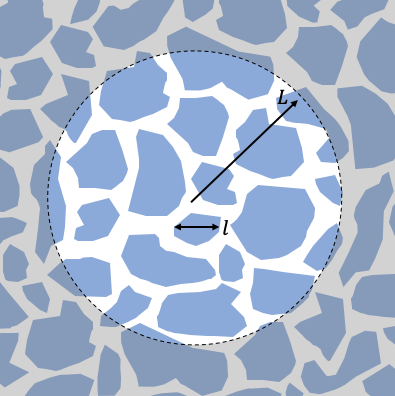
\includegraphics[width=0.4\linewidth]{figs/rev.png}
\caption{Schematic of a \gls{rev} in a multiphase domain. The \gls{rev} has characteristic dimension \(L\), while the pore scale has characteristic dimension \(l\).}
\label{fig:rev}
\end{figure}

\noindent Several important notational definitions are needed. Consider a generic field \(\Phi\) in a multi-phase domain. In an approach very similar to the temporal averaging of the Navier-Stokes equations to obtain the \gls{rans} equations, represent \(\Phi\) as the sum of its average \(\la\Phi\ra\) and a fluctuating component \(\hat{\Phi}\) with zero average,

\beq
\label{eq:PM_back}
\Phi=\la\Phi\ra+\hat{\Phi}\ ,
\eeq

\noindent where \(\la\Phi\ra\) is defined as

\beq
\label{eq:AverageDef}
\la\Phi\ra\equiv\frac{1}{\volume}\int_{\volume}\Phi d\volume ,
\eeq

\noindent and \(\volume\) indicates a volume. Eq. \eqref{eq:AverageDef} represents the average over all phases. An average over the \(k\) phase is defined as

\beq
\label{eq:AvgDef2}
\la\Phi\ra^k\equiv\frac{1}{\volume_k}\int_{\volume_k}\Phi d\volume\ ,
\eeq

\noindent where \(\volume_k\) is the volume occupied by the \(k\) phase. In order to characterize the distribution of phases in the \gls{rev}, a phase function \(f_k\) is defined as

\beq
\label{eq:PhaseFunction}
f_k=\begin{dcases} 1 & \textrm{in phase $k$}\\ 0 & \textrm{not in phase $k$} \end{dcases}\ .
\eeq

\noindent \(\Phi_k\) represents the value of \(\Phi\) in the \(k\) phase, 

\beq
\label{eq:KPhaseDef}
\Phi_k\equiv\Phi f_k\ ,
\eeq

\noindent while \(\la\Phi_k\ra\) indicates an average of \(\Phi_k\) over all phases,

\beq
\label{eq:PhaseAverage}
\la\Phi_k\ra\equiv\frac{1}{\volume}\int_{\volume}\Phi f_kd\volume\ ,
\eeq

\noindent and \(\la\Phi_k\ra^k\) indicates an average of \(\Phi_k\) over the \(k\) phase,

\beq
\label{eq:IntrinsicPhaseAverage}
\la\Phi_k\ra^k\equiv\frac{1}{\volume_k}\int_{\volume_k}\Phi f_kd\volume\ .
\eeq

\noindent \(\la\Phi_k\ra\) is referred to as the ``extrinsic,'' or ``superficial'' average over phase \(k\), while \(\la\Phi_k\ra^k\) is referred to as the ``intrinsic,'' or ``interstitial'' average over phase \(k\). For fluid flowing in a packed bed, the fluid velocity averaged over the fluid phase represents an intrinsic average. The fluid velocity averaged over both phases, as if the fluid were flowing at the same mass flow rate in an empty bed, represents an extrinsic average. This difference between extrinsic and intrinsic averages plays an important role in the derivation of the porous media equations. 

The porosity \(\epsilon\) for phase \(k\) is the fraction of the total volume occupied by phase \(k\),

\beq
\label{eq:PorosityAvg}
\epsilon_k\equiv\frac{\volume_k}{\volume}\ .
\eeq

\noindent This work considers two-phase fluid-solid domains; an \(f\) subscript refers to the fluid phase and an \(s\) subscript refers to the solid phase. The notational convention used throughout is that \(\epsilon_f\equiv\epsilon\) represents the porosity of the fluid and \(\epsilon_s\equiv1-\epsilon\) represents the porosity of the solid. Models for porosity are described in Section \ref{sec:Porosity}. 

Combining Eqs. \eqref{eq:PhaseAverage}--\eqref{eq:PorosityAvg} provides the relationship between intrinsic and extrinsic averages,

\beq
\label{eq:DupuitF}
\la\Phi_k\ra=\epsilon_k\la\Phi_k\ra^k\ .
\eeq

\noindent Applying Eq. \eqref{eq:DupuitF} to the extrinsic and intrinsic velocities discussed in the preceding paragraphs,

\beq
\label{eq:DupuitForchiemer}
\vec{v}=\epsilon\vec{V}\ ,
\eeq

\noindent where \(\vec{v}\) is the extrinsic fluid velocity, also referred to as the superficial velocity. \(\vec{V}\) is the intrinsic fluid velocity, also referred to as the interstitial velocity. 

Appendix \ref{sec:PorousMediaMath} provides mathematical identities relating the spatial averages of gradients to the gradients of spatial averages and the spatial averages of time derivatives to the time derivatives of spatial averages. The key requirement for the use of these identities is that a spatial average be independent of the size of the volume over which it is averaged. Similar restrictions abound in other forms of statistical analysis, such as in requirements of large numbers of coin tosses to accurately estimate the probability of landing tails-up. With the length scales defined in Fig.\ \ref{fig:rev}, this requirement can be expressed as

\beq
\label{eq:LengthReqs}
l\ll L\ .
\eeq

\noindent For packed beds of spherical pebbles, \(l\) is usually taken as the pebble diameter \(d_p\) or the hydraulic diameter \(D\), which is proportional to \(d_p\). The \gls{rev} scale \(L\) is larger than \(l\) but smaller than the largest bed dimension. The extrinsic and intrinsic averages are functions of space; the average at a location \(\vec{x}\) is interpreted as an average over a \gls{rev} with characteristic dimension \(L\) centered about \(\vec{x}\). A Taylor series analysis performed in Appendix \ref{sec:PorousMediaMath} shows that the assumption that averages are independent of the size of the \gls{rev} is accurate to \(\mathcal{O}(l/L)^2\).

The spatially homogenized conservation equations are now derived using the identities in Appendix \ref{sec:PorousMediaMath}; any notation not explicitly defined here is defined in Appendix \ref{sec:PorousMediaMath}. It is assumed throughout that thermal and pressure gradients are small relative to velocity gradients such that fluctuations in density, thermal conductivity, and isobaric specific heat capacity are much smaller than fluctuations in velocity and can hence be assumed zero \cite{gray}. It is also assumed that the solid-fluid interface is stationary such that \(\vec{V}=\vec{w}\) on the interface and \(\vec{w}=0\), where \(\vec{w}\) is the interface velocity. For conciseness, these assumptions are made implicitly while progressing through the derivation, though explicit tracking of these additional terms may be found elsewhere \cite{novak_manual}.

The identities derived in Appendix \ref{sec:PorousMediaMath} relate spatial averages of time derivatives, gradients, and products to time derivatives, gradients, and products of spatial averages. For example, Eq. \eqref{eq:TimeAvgDerivativeb} relates the spatial average of a time derivative to the time derivative of a spatial average plus an integral over the phase interface. The use of each particular identity from Appendix \ref{sec:PorousMediaMath} should be clear from the nature of each kernel, though subtle details will be noted as appropriate.

%Beginning with the mass conservation equation in Eq. \eqref{eq:ContinuityNonPorous}, the time derivative is averaged using Eqs. \eqref{eq:TimeAvgDerivativeb} and \eqref{eq:Dispersion}, while the advective term is averaged using Eqs. \eqref{eq:AvgGrdGrdAvga} and Eq. \eqref{eq:Dispersion}, giving

Spatial averaging of the mass conservation equation in Eq. \eqref{eq:ContinuityNonPorous} gives

\beq
\label{eq:PorousMass1}
\frac{\partial\left(\epsilon\la\rho_f\ra^f\right)}{\partial t}+\nabla\cdot\left(\epsilon\la\rho_f\ra^f\la\vec{V}_f\ra^f\right)=0\ ,
\eeq

\noindent where Eq. \eqref{eq:DupuitF} was used. For notational simplicity, Eq. \eqref{eq:PorousMass1} is rewritten as

\beq
\label{eq:PorousMass}
\frac{\partial(\epsilon\rho_f)}{\partial t}+\nabla\cdot(\epsilon\rho_f\vec{V})=0\ ,
\eeq

\noindent where \(\rho_f\) represents the intrinsic average of fluid density and \(\vec{V}\) represents the intrinsic average of fluid velocity.

%Moving next to the momentum conservation equation in Eq. \eqref{eq:NSFullForm}, the time derivative is averaged using Eqs. \eqref{eq:TimeAvgDerivativeb} and \eqref{eq:Dispersion}, while the advective, normal stress and deviatoric stress terms are averaged using Eqs. \eqref{eq:AvgGrdGrdAvg} and \eqref{eq:Dispersion3}, giving

Spatial averaging of the momentum conservation equation in Eq. \eqref{eq:NSFullForm} gives

\beqa
\label{eq:MomFirstStep}
&\frac{\partial(\epsilon\la\rho_f\ra^f\la\vec{V}_f\ra^f)}{\partial t}+\nabla\cdot\left(\epsilon\la\rho_f\ra^f\la\vec{V}_f\ra^f\la\vec{V}_f\ra^f+\la\rho_f\ra^f\la\hat{\vec{V}}_f\hat{\vec{V}}_f\ra\right)=-\epsilon\nabla\la P_f\ra^f+\\
&\hspace{0.5cm}\nabla\cdot\la\tau_f\ra+\frac{1}{\volume}\int_{S_i}\tau_f\hat{n}_fdS-\frac{1}{\volume}\int_{S_i}\left(\hat{P}_f-\la\rho_f\ra^f\hat{\phi}_{g,f}\right)\hat{n}_fdS-\epsilon\la\rho_f\ra^f\nabla\la\phi_{g,f}\ra^f\ .
\eeqa

\noindent The source term \(-\rho_f\nabla\phi_{g,f}\) is related to the gravitational potential \(\phi_{g,f}\) as

\beq
\label{eq:GravitationalPotential}
\nabla\phi_{g,f}\equiv -g\vec{e}_z\ ,
\eeq

%\noindent where averaging was performed using Eqs. \eqref{eq:AvgGrdGrdAvgb} and \eqref{eq:Dispersion}, with 

\noindent Terms containing the fluctuation of \(\vec{g}\) are set to zero because the gravitational acceleration vector is constant. 

The advective and deviatoric stress terms were averaged using Eq. \eqref{eq:AvgGrdGrdAvga}, but the normal stress term was averaged using Eq. \eqref{eq:AvgGrdGrdAvgb}. The different form used for the normal stress is required to correctly enforce that porosity gradients in stagnant fluid systems do not spontaneously induce flows \cite{kececioglu}. For a Newtonian fluid, \(\nabla\cdot\la\tau_f\ra\) becomes

\beqa
\label{eq:DeviatoricStressApprox}
\nabla\cdot\la\tau_f\ra=\nabla\cdot\left\{\la\mu_f\ra\left\lbrack\nabla\la\vec{V}_f\ra+(\nabla\la\vec{V}_f\ra)^T-\frac{2}{3}\nabla\cdot\la\vec{V}_f\ra\textbf{I}\right\rbrack\right\}\ ,
\eeqa

\noindent where the surface integral terms arising from Eq. \eqref{eq:AvgGrdGrdAvg} are zero due to the no-slip condition at phase interfaces. The \(\tau_f\hat{n}_f\) integral in Eq. \eqref{eq:MomFirstStep} represents the average viscous drag. This term can be expressed in terms of the difference in intrinsic phase velocity difference since the viscous stress is zero if neither phase is moving. Assuming a second-order expansion, the drag term is written as

\beqa
\label{eq:StressApprox}
&\frac{1}{\volume}\int_{S_i}\tau_f\cdot\hat{n}_fdS=\la\mu_f\ra\epsilon\mathscr{A}\left(\la\vec{V}_s\ra^s-\la\vec{V}_f\ra^f\right)+\\
&\hspace{0.5cm}\la\mu_f\ra\epsilon\mathscr{B}:\left(\la\vec{V}_s\ra^s-\la\vec{V}_f\ra^f\right)\cdot\left(\la\vec{V}_s\ra^s-\la\vec{V}_f\ra^f\right)\ ,
\eeqa

\noindent where \(\mathscr{A}\) is a second-order tensor and \(\mathscr{B}\) a third-order tensor. The \(\la\hat{\vec{V}}_f\hat{\vec{V}}_f\ra\) term in Eq. \eqref{eq:MomFirstStep} will only be zero if the fluid moves at the same velocity as the fluid-solid interface. This requirement can also be expressed as a two-term expansion,

\beq
\label{eq:MechanicalApprox}
\la\hat{\vec{V}}_f\hat{\vec{V}}_f\ra=\epsilon\mathscr{C}\cdot\left(\la\vec{V}_s\ra^s-\la\vec{V}_f\ra^f\right)+\epsilon\mathscr{L}:\left(\la\vec{V}_s\ra^s-\la\vec{V}_f\ra^f\right)\left(\la\vec{V}_s\ra^s-\la\vec{V}_f\ra^f\right)\ ,
\eeq

\noindent where \(\mathscr{C}\) is a third-order tensor and \(\mathscr{L}\) is a fourth-order tensor. Because \(\la\hat{\vec{V}}_f\hat{\vec{V}}_f\ra\) is symmetric, both of these tensors must be symmetric in their first two indices, and \(\mathscr{L}\) also in the last two indices. 

One more constitutive relationship is required to close the momentum equation. The fluctuating pressure and gravitational field are nonzero perturbations that can still satisfy \(\nabla\la P_f\ra^f+\la\rho_f\ra^f\nabla\la\phi_{g,f}\ra^f=0\), such as when the fluid is hydrostatic. Therefore, expressing this term as a second order expansion gives

\beqa
\label{eq:PressureApprox}
\frac{1}{\volume}\int_{S_i}\left(\hat{P}_f+\la\rho_f\ra^f\hat{\phi}_{g,f}\right)\hat{n}_fdS= \epsilon\mathscr{E}\cdot\left(\nabla\la P_f\ra^f+\la\rho_f\ra^f\nabla\la\phi_{g,f}\ra^f\right)+\hspace{1cm}\\
\epsilon\mathscr{M}:\left(\nabla\la P_f\ra^f+\la\rho_f\ra^f\nabla\la\phi_{g,f}\ra^f\right)\left(\nabla\la P_f\ra^f+\la\rho_f\ra^f\nabla\la\phi_{g,f}\ra^f\right)\ ,
\eeqa

\noindent where \(\mathscr{E}\) is a second-order tensor and \(\mathscr{M}\) is a third-order tensor that is symmetric in its second and third indices. Inserting Eqs.  \eqref{eq:DeviatoricStressApprox}--\eqref{eq:PressureApprox} into Eq. \eqref{eq:MomFirstStep} gives the porous media momentum equation for a Newtonian fluid,

\beqa
\label{eq:MomEqnStep2}
\frac{\partial(\epsilon\la\rho_f\ra^f\la\vec{V}_f\ra^f)}{\partial t}+\nabla\cdot\left\lbrack\epsilon\la\rho_f\ra^f\la\vec{V}_f\ra^f\la\vec{V}_f\ra^f+\epsilon\la\rho_f\ra^f\mathscr{C}\cdot\left(\la\vec{V}_s\ra^s-\la\vec{V}_f\ra^f\right)\right\rbrack+\hspace{1.25cm}\\
\nabla\cdot\left\lbrack\epsilon\la\rho_f\ra^f\mathscr{L}:\left(\la\vec{V}_s\ra^s-\la\vec{V}_f\ra^f\right)\left(\la\vec{V}_s\ra^s-\la\vec{V}_f\ra^f\right)\right\rbrack=\hspace{1cm}\\
\nabla\cdot\left\{\la\mu_f\ra\left\lbrack\nabla\la\vec{V}_f\ra+(\nabla\la\vec{V}_f\ra)^T-\frac{2}{3}\nabla\cdot\la\vec{V}_f\ra\textbf{I}\right\rbrack\right\}+\hspace{0.75cm}\\
\la\mu_f\ra\epsilon\mathscr{A}\left(\la\vec{V}_s\ra^s-\la\vec{V}_f\ra^f\right)+\la\mu_f\ra\epsilon\mathscr{B}:\left(\la\vec{V}_s\ra^s-\la\vec{V}_f\ra^f\right)\cdot\left(\la\vec{V}_s\ra^s-\la\vec{V}_f\ra^f\right)-\hspace{0.5cm}\\
\epsilon\left(\textbf{I}+\mathscr{E}\right)\cdot\left(\nabla\la P_f\ra^f+\la\rho_f\ra^f\nabla\la\phi_{g,f}\ra^f\right)-\hspace{0.25cm}\\
\epsilon\mathscr{M}:\left(\nabla\la P_f\ra^f+\la\rho_f\ra^f\nabla\la\phi_{g,f}\ra^f\right)\left(\nabla\la P_f\ra^f+\la\rho_f\ra^f\nabla\la\phi_{g,f}\ra^f\right)\ .
\eeqa

\noindent Models for all of the tensors that appear in Eq. \eqref{eq:MomEqnStep2} do not exist. To obtain a tractable momentum equation, mechanical effects of the solid on the fluid are neglected such that \(\mathscr{C}=\textbf{0}\) and \(\mathscr{L}=\textbf{0}\). Second-order effects of the pressure and gravitational forces are also neglected such that \(\mathscr{M}=\textbf{0}\). Both of these approximations are valid for relatively slow flows \cite{gray}. Eq. \eqref{eq:MomEqnStep2} then becomes

\beqa
\label{eq:MomEqnStep3a}
\frac{\partial(\epsilon\la\rho_f\ra^f\la\vec{V}_f\ra^f)}{\partial t}+\nabla\cdot\left(\epsilon\la\rho_f\ra^f\la\vec{V}_f\ra^f\la\vec{V}_f\ra^f\right)=-W\la\rho_f\ra^f\la\vec{V}_f\ra^f+\hspace{1cm}\\
\epsilon\nabla\la P_f\ra^f+\nabla\cdot\left(\tilde{\mu}\nabla\langle\vec{V}_f\rangle^f\right)+\epsilon\la\rho_f\ra^f\nabla\la\phi_{g,f}\ra^f\ ,
\eeqa

\noindent where the viscous term in Eq. \eqref{eq:MomEqnStep2} has been replaced by a distributed loss friction term that captures the  \(\epsilon\la\mu_f\ra\mathscr{A}(\textbf{I}+\mathscr{E})^{-1}\) and \(\epsilon\la\mu_f\ra\mathscr{B}(\textbf{I}+\mathscr{E})^{-1}\) terms. The sum of these two terms (with \(\mathscr{A}\) divided by \(\la\rho_f\ra^f\) to obtain the proper units) is denoted as \(W\), a combined Darcy and Forchheimer friction factor. A distributed loss friction model is usually sufficient to capture the interphase drag because the length over which the deviatoric stress acts is on the order of several pore diameters \cite{kececioglu}. Models for \(W\) are described in Section \ref{sec:W}.

Some porous media models also include a Brinkman viscous stress term to allow no-slip \glspl{bc} to be applied on boundaries. Brinkman's model expresses the viscous stress term in Eq. \eqref{eq:DeviatoricStressApprox} as the sum the Darcy and Forchheimer drag discussed previously plus a velocity laplacian with effective viscosity \(\tilde{\mu}\); such a term is shown in Eq. \eqref{eq:MomEqnStep3a} \cite{nield,auwerda_2011,tecdoc1163}. Brinkman's model does not have the same validation basis as either Darcy's or Forchheimer's drag terms, and is generally thought to only be applicable for \(\epsilon>0.8\). At lower porosities, the solid matrix impedes direct transfer of momentum due to viscous forces and the majority of stresses are communicated via pressure \cite{nield}. For completeness, a Brinkman model is shown in the spatially homogenized momentum equation, though the term is usually negligibly small for high Reynolds number reactor applications. Models for \(\tilde{\mu}\) are described in Section \ref{sec:BrinkmanMu}.

For notational simplicity, Eq. \eqref{eq:MomEqnStep3a} is written as

\beq
\label{eq:MomEqnStep3}
\frac{\partial(\epsilon\rho_f\vec{V})}{\partial t}+\nabla\cdot(\epsilon\rho_f\vec{V}\vec{V})=-W\rho_f\vec{V}+\epsilon\nabla P+\nabla\cdot(\tilde{\mu}\nabla\vec{V})+\epsilon\rho_f\vec{g}\ ,
\eeq

\noindent where \(\rho_f\) and \(\vec{V}\) have the same interpretation as in Eq. \eqref{eq:PorousMass} and \(P\) represents the intrinsic average of pressure.

Only the energy equations remain to be spatially homogenized. Scaling analysis in Section \ref{sec:NonDim} justifies the omission of the viscous heating terms\mdash the \(\nabla\cdot(\vec{V}\tau)\) term in Eq. \eqref{eq:EnergyNonPorous} and the \(\tau\colon\nabla\vec{V}\) term in Eq. \eqref{eq:InternalEnergy}. Section \ref{sec:NonDim} also justifies neglecting the compression work term proportional to \(dP/dt\). Rather than carry the viscous heating and compression work terms through the derivation for completeness, notational simplicity motivates its omission at the beginning of this derivation. 

% For the total energy conservation in Eq. \eqref{eq:EnergyNonPorous}, the time derivative is averaged using Eqs. \eqref{eq:TimeAvgDerivativeb} and \eqref{eq:Dispersion}, while the advective and conductive terms are averaged using Eqs. \eqref{eq:AvgGrdGrdAvg} and \eqref{eq:Dispersion3}, giving

Spatial homogenization of the total energy conservation equation in Eq. \eqref{eq:EnergyNonPorous} gives

\beqa
\label{eq:Energy1}
&\frac{\partial(\epsilon\la\rho_f\ra^f\la E_f\ra^f)}{\partial t}+\nabla\cdot\left(\epsilon\la\rho_f\ra^f\la H_f\ra^f\la\vec{V}_f\ra^f+\la\rho_f\ra^f\la\hat{H}_f\hat{\vec{V}}_f\ra\right)=\nabla\cdot\left(\la k_f\ra^f\epsilon\nabla\la T_f\ra^f\right)+\\
&\hspace{0.5cm}\nabla\cdot\left( \frac{\la k_f\ra^f}{\volume}\int_{S_i}\hat{T}\hat{n}_fdS\right)+\frac{1}{\volume}\int_{S_i}k_f\nabla T_f\cdot\hat{n}_fdS+\epsilon\la\rho_f\ra^f\la\vec{V}_f\ra^f\cdot\la\vec{g}\ra^f+\la \dot{q}_f\ra\ .
\eeqa

% The gravitational power and volumetric heat source terms were transformed using Eq. \eqref{eq:Dispersion}. 

\noindent The surface integral with integrand \(\hat{T}_f\hat{n}_f\) represents the ``tortuosity heat flux.'' The tortuosity heat flux is often very small because convection dominates conduction, and hence is neglected \cite{nakayama}. The surface integral with integrand \(k_f\nabla T_f\cdot\hat{n}_f\) represents the average heat flux at the phase boundary, which is represented by a convective flux closure as

\beq
\label{eq:ConvecCoolClosure}
\frac{1}{\volume}\int_{S_i}k_f\nabla T_f\hat{n}_fdS=\alpha\left(\la T_s\ra^s-\la T_f\ra^f\right)\ ,
\eeq

\noindent where \(\alpha\) is the convective heat transfer coefficient and \(\la T_s\ra^s\) is the intrinsic phase-averaged solid surface temperature. To obtain the correct units, \(\alpha\) represents the heat transfer coefficient \(h_c\) multiplied by \(a_w\),

\beq
\label{eq:Alpha}
\alpha\equiv a_wh_c\ ,
\eeq

\noindent where \(a_w\) is the wetted area per unit length,

\beq
\label{eq:AwLimit}
a_w=\lim_{\delta\ \to\ 0} \frac{\text{wetted area in domain of length } \delta}{\text{volume of domain of length }\delta}\ .
\eeq

\noindent Models for \(\alpha\) are described in Section \ref{sec:alpha}. Neglecting the tortuosity heat flux and inserting Eq. \eqref{eq:ConvecCoolClosure} into Eq. \eqref{eq:Energy1}, the total energy conservation equation becomes

\beqa
\label{eq:Energy2}
&\frac{\partial(\epsilon\la\rho_f\ra^f\la E_f\ra^f)}{\partial t}+\nabla\cdot\left(\epsilon\la\rho_f\ra^f\la H_f\ra^f\la\vec{V}_f\ra^f+\la\rho_f\ra^f\la\hat{H}_f\hat{\vec{V}}_f\ra\right)=\\
&\hspace{1cm}\nabla\cdot\left(\la k_f\ra^f\epsilon\nabla\la T_f\ra^f\right)+\epsilon\la\rho_f\ra^f\la\vec{V}_f\ra^f\cdot\la\vec{g}\ra^f+\alpha\left(\la T_s\ra^s-\la T_f\ra^f\right)+\la \dot{q}_f\ra\ .
\eeqa

\noindent Before introducing the final closure for the \(\nabla\cdot\left(\la\rho_f\ra^f\la\hat{H}_f\hat{\vec{V}}_f\ra\right)\) term, which will be shared by the spatially homogenized internal energy equation, first homogenize the internal energy equation in Eq. \eqref{eq:InternalEnergy}, giving

\beqa
\label{eq:PorousT}
\epsilon\la\rho_f\ra^f\la C_{p,f}\ra^f\frac{\partial\la T_f\ra^f}{\partial t}+\epsilon\la\rho_f\ra^f\la C_{p,f}\ra^f\la\vec{V}_f\ra^f\cdot\nabla\la T_f\ra^f+\la\rho_f\ra^f\la C_{p,f}\ra^f\la\hat{\vec{V}}_f\cdot\hat{\nabla T_f}\ra=\hspace{0.5cm}\\
\nabla\cdot\left(\la k_f\ra^f\epsilon\nabla\la T_f\ra^f\right)+\alpha\left(\la T_s\ra^s-\la T_f\ra^f\right)+\la \dot{q}_f\ra\ ,
\eeqa

\noindent where the spatial homogenization performed for terms shared by the total energy and internal energy equations have been inserted. The tortuosity heat flux term has also been neglected.

Eqs. \eqref{eq:Energy2} and \eqref{eq:PorousT} still leave one term that requires closure\mdash the \(\nabla\cdot(\la\rho_f\ra^f\la\hat{H}_f\hat{\vec{V}}_f\ra)\) term in Eq. \eqref{eq:Energy2} and the \(\la\rho_f\ra^f\la C_{p,f}\ra^f\la\hat{\vec{V}}_f\cdot\hat{\nabla T_f}\ra\) term in Eq. \eqref{eq:PorousT}. These two terms represent enhancements in advective energy transport due to the porous structure, a phenomenon referred to as ``thermal dispersion.'' Thermal dispersion accounts for the effects of changes in flow direction caused by solid obstructions, recirculation flows within the pores, and eddy diffusion in turbulence. Thermal dispersion is represented with a gradient diffusion model,

\beq
\label{eq:ThermalDispersion}
\la\rho_f\ra^f\la C_{p,f}\ra^f\la\hat{\vec{V}}_f\cdot\hat{\nabla T_f}\ra= -\nabla\cdot(\tilde{\kappa}_f\nabla \la T_f\ra^f)\ ,
\eeq

\noindent where \(\tilde{\kappa}_f\) is the thermal dispersion conductivity, which is in general a second-order tensor \cite{nakayama}. While Eq. \eqref{eq:ThermalDispersion} is shown in terms of the dispersion kernel in Eq. \eqref{eq:PorousT}, a similar interpretation exists for the dispersion kernel in Eq. \eqref{eq:Energy2}. The effective fluid thermal conductivity \(\kappa_f\) represents the sum of molecular and dispersion conductivity, 

\beq
\label{eq:KappaFluidDef1}
\kappa_f\equiv\epsilon k_f+\tilde{\kappa}_f\ .
\eeq

\noindent Models for \(\kappa_f\) are described in Section \ref{sec:Kappa}. Inserting Eqs. \eqref{eq:ThermalDispersion} and \eqref{eq:KappaFluidDef1} into Eqs. \eqref{eq:Energy2} and \eqref{eq:PorousT} gives

\beqa
\label{eq:Energy3}
&\frac{\partial(\epsilon\la\rho_f\ra^f\la E_f\ra^f)}{\partial t}+\nabla\cdot\left(\epsilon\la\rho_f\ra^f\la H_f\ra^f\la\vec{V}_f\ra^f\right)=\\
&\hspace{1cm}\nabla\cdot\left(\kappa_f\nabla\la T_f\ra^f\right)+\epsilon\la\rho_f\ra^f\la\vec{V}_f\ra^f\cdot\la\vec{g}\ra^f+\alpha\left(\la T_s\ra^s-\la T_f\ra^f\right)+\la \dot{q}_f\ra\ ,
\eeqa

\noindent and

\beqa
\label{eq:PorousT1}
\epsilon\la\rho_f\ra^f\la C_{p,f}\ra^f\frac{\partial\la T_f\ra^f}{\partial t}+\epsilon\la\rho_f\ra^f\la C_{p,f}\ra^f\la\vec{V}_f\ra^f\cdot\nabla\la T_f\ra^f=\hspace{1cm}\\
\nabla\cdot\left(\kappa_f\nabla\la T_f\ra^f\right)+\alpha\left(\la T_s\ra^s-\la T_f\ra^f\right)+\la \dot{q}_f\ra\ .
\eeqa

\noindent For notational simplicity, Eqs. \eqref{eq:Energy3} and \eqref{eq:PorousT1} are rewritten as

\beq
\label{eq:EnergyBalance7}
\frac{\partial (\epsilon\rho_f E_f)}{\partial t}+\nabla\cdot(\epsilon H_f\rho_f\vec{V})=\nabla\cdot(\kappa_f\nabla T_f)+\epsilon\rho_f \vec{g}\cdot\vec{V}+\alpha(T_s-T_f)+\dot{q}_f\ ,
\eeq

\noindent and

\beq
\label{eq:EnergyBalanceT}
\epsilon\rho_fC_{p,f}\frac{\partial T_f}{\partial t}+\epsilon\rho_fC_{p,f}\vec{V}\cdot\nabla T_f=\nabla\cdot(\kappa_f\nabla T_f)+\alpha(T_s-T_f)+\dot{q}_f\ ,
\eeq

\noindent where \(\rho_f\) and \(\vec{V}\) have the same interpretation as in Eq. \eqref{eq:PorousMass}, \(E_f\) represents the intrinsic average of total energy, \(H_f\) represents the intrinsic average of total enthalpy, \(T_f\) represents the intrinsic average of fluid temperature, \(T_s\) represents the intrinsic average of the solid surface temperature, \(\dot{q}_f\) represents the extrinsic average of the fluid volumetric heat source, and \(C_{p,f}\) represents the intrinsic average of the fluid isobaric specific heat capacity.

The conservation of solid energy equation can be derived by spatially homogenizing the heat equation using the identities in Appendix \ref{sec:PorousMediaMath}. A simpler, but equivalent, approach instead sets \(\vec{V}\) to zero in Eq. \eqref{eq:EnergyBalanceT}, replaces all \(f\) subscripts with \(s\) subscripts, and substitutes \(1-\epsilon\) for \(\epsilon\), giving

\beq
\label{eq:SolidPorous}
(1-\epsilon)\rho_sC_{p,s}\frac{\partial T_s}{\partial t}-\nabla\cdot(\kappa_s\nabla T_s)+\alpha(T_s-T_f)-\dot{q}_s=0\ ,
\eeq

\noindent where \(\kappa_s\) represents the effective solid thermal conductivity, \(\rho_s\) represents the intrinsic average of the solid density, \(C_{p,s}\) represents the intrinsic average of the solid isobaric specific heat capacity, and \(\dot{q}_s\) represents the extrinsic average of the solid volumetric heat source. \(\kappa_s\) captures the combined dispersion effects of solid-to-solid radiation \(\kappa_\text{radiation}\), solid-fluid-solid conduction \(\kappa_\text{conduction}\), and solid-to-solid conduction \(\kappa_\text{contact}\),

\beq
\label{eq:Kappa}
\kappa_s\equiv\kappa_{\textrm{radiation}}+\kappa_{\textrm{fluid conduction}}+\kappa_{\textrm{solid conduction}}\ .
\eeq

\noindent Thermal equilibrium is often assumed for geophysical applications, and is even the default in FLUENT's porous media model \cite{fluent}. The inclusion of unique energy conservation equations for the phases with the convective heat transfer term in Eq. \eqref{eq:ConvecCoolClosure} is essential for modeling of reactor systems due to the volumetric heat sources and the different material properties of the phases \cite{becker,novak_sana}.

In summary, the mass, momentum, and energy conservation equations were spatially homogenized by averaging over a \gls{rev} consisting of a mixture of fluid and solid. Several different models are considered for the macroscale, motivated by the wide range in \gls{th} conditions in \glspl{pbr} and the improved nonlinear convergence behavior that can be obtained by neglecting certain physics kernels. The inviscid Navier-Stokes model represented by Eqs. \eqref{eq:PorousMass}, \eqref{eq:MomEqnStep3} with \(\tilde{\mu}=0\), and \eqref{eq:EnergyBalance7} has two solutions as the Mach number tends to zero\mdash an incompressible limit and an acoustic limit. For nearly incompressible fluids such as molten salts, solution of a compressible model may be an inaccurate representation of the incompressible solution because the incompressible limit is a singular limit of the compressible flow equations \cite{guillard}. A model that neglects the compression work term may provide a better representation of the incompressible solution and enable vastly improved numerical convergence.

Two different models are used depending on the flow conditions and desired level of accuracy\mdash a Navier-Stokes model and a friction-dominated model. The spatially homogenized Navier-Stokes equations on the macroscale are

\begin{subequations}
\label{eq:PorousEquations}
\begin{align}
\label{eq:PMass}\massconservation\ ,\\
\label{eq:PMom}\momentumconservation\ ,\\
\label{eq:PEnergy}\fluidenergyconservation\ ,\\
\label{eq:PSEnergy}\solidenergyconservation\ .
\end{align}
\end{subequations}

\noindent Eq. \eqref{eq:PorousEquations} is referred to here as the ``Navier-Stokes model.'' All terms in Eqs. \eqref{eq:PMass}--\eqref{eq:PEnergy} have the same form as the local compressible Navier-Stokes equations except the Brinkman stress term, which has the same local form as the incompressible Navier-Stokes viscous stress in order to match literature closures for \(\tilde{\mu}\). An inviscid flow model can be obtained as a simplification of Eq. \eqref{eq:PorousEquations} with \(\tilde{\mu}=0\).

For slowly-evolving, low Reynolds number flows, several additional approximations can be made to simplify Eq. \eqref{eq:PorousEquations}. Momentum conservation is assumed dominated by friction effects such that changes in pressure are instantaneously reflected as changes in momentum. The total derivative of momentum in Eq. \eqref{eq:PMom} is set to zero, giving a pseudo-steady momentum equation. The Brinkman viscosity is also set to zero. Substituting this pseudo-steady momentum equation into the mass conservation in Eq. \eqref{eq:PMass} then gives a pressure Poisson equation. Further, compression work is assumed negligible such that energy conservation is well approximated by Eq. \eqref{eq:EnergyBalanceT}. Together, these assumptions give,

\begin{subequations}
\label{eq:PrimitiveEqns}
\begin{align}
\label{eq:PMass2}
\legacymass\ ,\\
\label{eq:PMom2}
\legacymomentum\ ,\\
\label{eq:PEnergy2}
\legacyfluidenergy\ ,\\
\label{eq:PSEnergy2}
\legacysolidenergy\ .
\end{align}
\end{subequations}

\noindent Eq. \eqref{eq:PrimitiveEqns} is referred to here as the ``friction-dominated model.'' This friction-dominated model has been widely used for the analysis of \glspl{pbr} \cite{hossain, nouri, tecdoc1163}.  

Pebbles move continuously through the bed in online refueling operation. Depending on the design, pebbles cycle between 2 and 10 times over a period of several years. The velocity of these motions is orders of magnitude smaller than the fluid velocity. The kinetic energy of pebbles in fluidized beds such as liquid salt systems are also negligibly small \cite{mardus_hall}. Therefore, porosity is assumed independent of time such that it is moved outside the time derivatives in Eqs. \eqref{eq:PorousEquations} and \eqref{eq:PrimitiveEqns}.

As will be discussed at greater length in Chapter \ref{sec:ph}, Eqs. \eqref{eq:PorousEquations} and \eqref{eq:PrimitiveEqns} may be solved for a number of different solution variables to enable general simulation of compressible and incompressible flows, flexible application of the \glspl{bc} described in Section \ref{sec:BCs}, and better numerical convergence in the presence of certain material discontinuities \cite{hauke_1998}. These solution variables are the primitive interstitial set \(P\), \(\vec{V}\), and \(T_f\); the primitive superficial set \(P\), \(\vec{v}\), and \(T_f\); the mixed interstitial set \(P\), \(\rho_f\vec{V}\), and \(T_f\); the mixed superficial set \(P\), \(\rho_f\vec{v}\), and \(T_f\); and the conservative interstitial set \(\rho_f\), \(\rho_f\vec{V}\), and \(\rho_fE_f\).

\subsection{Non-Dimensional Analysis}
\label{sec:NonDim}

This section presents a brief scaling analysis of the momentum and energy conservation equations to justify omission of the viscous heating term from Eqs. \eqref{eq:PorousEquations} and \eqref{eq:PrimitiveEqns} and the compression work term from Eq. \eqref{eq:PrimitiveEqns}. For notational simplicity, this scaling analysis is performed starting from the local conservation equations because small terms were neglected at the outset of the spatial homogenization procedure, rather than carried through to be neglected at the conclusion.

Scaling analysis begins with the 1-D form of momentum conservation in Eq. \eqref{eq:NSFullForm}. Define the following nondimensional quantities,

\beq
\label{eq:NondimensionalQuantities}
t^+=\frac{t}{L/V_o},\quad V^+=\frac{V}{V_o},\quad P^+=\frac{P}{\rho_oV_o^2},\quad x^+=\frac{x}{L},\quad g^+=\frac{g}{g_o}\ ,
\eeq

\noindent where a \(+\) superscript indicates a nondimensional quantity. Inserting Eq. \eqref{eq:NondimensionalQuantities} into the 1-D form of Eq. \eqref{eq:NSFullForm} with constant viscosity and dividing through by the coefficient on the advective term gives

\beqa
\label{eq:NondimensionalNS2}
\frac{dV^+}{dx^+}=&\ \frac{Lg_o}{V_o^2}g^+-\frac{\partial P^+}{\partial x^+}+\frac{1}{Re}\frac{\partial}{\partial {x^+}}\left(\diamond\right)\ ,
\eeqa

\noindent where the viscous term is represented symbolically as \(\diamond\) and \(Re\) is the Reynolds number. For a generic porous medium characterized by two different velocity scales \(v\) and \(V\) and two different length scales \(d_p\) and \(D\), there are many manners in which the Reynolds number can be defined. The two most common definitions are

\begin{subequations}
\label{eq:RePorousGeneral}
\begin{align}
\label{eq:RePorousGeneralA}
Re=&\ \frac{\rho \|\vec{v}\|d_p}{\mu}\ ,\\
\label{eq:RePorousGeneralB}
Re_h=&\ \frac{\rho \|\vec{V}\|D}{\mu}\ .
\end{align}
\end{subequations}

\noindent Both Eqs. \eqref{eq:RePorousGeneralA} and \eqref{eq:RePorousGeneralB} are used throughout this work depending on whether the domain in question is porous or open, respectively. 

Non-dimensionalization of the energy conservation equation is performed beginning from the 1-D form of Eq. \eqref{eq:InternalEnergy} with the volumetric heat source omitted for simplicity. In addition to Eq. \eqref{eq:NondimensionalQuantities}, define

\beq
\label{eq:Nondim11}
T^+=\frac{T}{\Delta T}\ .
\eeq

\noindent Inserting Eqs. \eqref{eq:NondimensionalQuantities} and \eqref{eq:Nondim11} into the 1-D form of Eq. \eqref{eq:InternalEnergy} with constant thermal conductivity and dividing through by the coefficient on the advective term gives

\beq
\label{eq:NondimensionalTemperatureEqn}
\frac{dT^+}{dt^+}-\beta Ec\ T^+\frac{dP^+}{dt^+}=\frac{Br}{Pe}(\diamond)-\frac{1}{Pe}\frac{\partial}{\partial x^+}\frac{\partial T^+}{\partial x^+}\ ,
\eeq

\noindent where the viscous power term is represented symbolically as \(\diamond\). \(Pe\) is the Peclet number, defined as

\beq
\label{eq:PecletDef}
Pe\equiv\frac{\rho C_{p}\|\vec{V}\|L}{k}\ ;
\eeq

%High-Prandtl number fluids, such as molten salts, at Reynolds number typical of reactor operation display greater heat transfer caused by turbulence than diffusion \cite{song}. 

\noindent\(Ec\) is the Eckert number, defined as

\beq
\label{eq:EcNumber}
Ec=\frac{\|\vec{V}\|^2}{C_{p}\Delta T}\ ;
\eeq

\noindent and \(Br\) is the Brinkman number, defined as

\beq
\label{eq:BrNumber}
Br=\frac{\mu \|\vec{V}\|^2}{k\Delta T}\ .
\eeq

\noindent Viscous heating is negligible if \(Br/Pe\ll1\) and compression work is negligible if \(\beta Ec\ll1\). Table \ref{table:TypicalData} provides estimates of these dimensionless numbers for five representative reactor designs\mdash the sodium-cooled \gls{pfbr}, the helium-cooled \gls{thtr}, the \gls{flibe}-cooled \gls{pbfhr}, the water-cooled \gls{ap1000}, and the CO$_2$-cooled \gls{agr}. For all five designs, both viscous heating and compression work are orders of magnitude less significant than energy advection and can therefore be neglected from the macroscale model.

While \(Re\gg1\) for most applications, the Brinkman viscous stress is retained in the macroscale model for completeness and application of no-slip \glspl{bc}. Likewise, \(Pe\gg1\) for all systems considered, but thermal energy conduction is retained in the macroscale model because the gradient diffusion model for thermal dispersion always requires a diffusive kernel.

\begin{table}[!h]
\caption{Operating conditions and approximate nondimensional numbers for representative nuclear reactor designs \cite{pfbr,pfbrTH,thtr_1990,pbfhr,ap1000,ap1000_2,nonbol}. All material properties are evaluated at the median of the operating temperature range. Temperatures are listed as ``inlet/outlet.''}
\centering
\begin{tabular}{|l |l l l l l|}
\hline\hline
 								& PFBR		& THTR 			& PB-FHR 				& AP-1000 			& AGR\Tstrut\Bstrut \\
\hline
 Coolant							& sodium			& helium				& \gls{flibe}				& water				& CO\textsubscript{2}\Tstrut\\
 Power (MW$_\text{th}$)				& 1250			& 750				& 236				& 3400				& 1623\\
 Fuel	 geometry							& assembly		& pebble				& pebble				& assembly			& assembly\Bstrut\\
 \hline
Pressure (\si{\mega\pascal})						& 0.1				& 4.0					& 0.1					& 15.5				& 4.1\Tstrut\\
Temperature(\si{\celsius})				& 400/550		& 250/750				& 600/700				& 280/325				& 340/640\\
Flowrate (\si{\kilo\gram\per\second})						& 6390			& 298				& 976				& 13700				& 4060\\
Velocity (\si{\meter\per\second})						& 4.8				& 12.0				& 0.4					& 4.8				& 1.6\Bstrut\\
 \hline
 \(D\) (mm)						& 5.0				& 26.0				& 13.0				& 11.7			& 38.0\Tstrut\\
 \(\rho\) (\si{\kilo\gram\per\cubic\meter})			& 840			& 2.5					& 2000				& 720			& 28\\
 \(\mu\) (\(10^{-5}\) Pa\(\cdot\)s)			& 25				& 3.9					& 680				& 8.7				& 3.4\\
 \(k\) (\si{\watt\per\meter\per\kelvin})					& 139			& 0.30				& 1.10				& 0.56			& 0.05\\
 \(C_p\) (\si{\joule\per\kilo\gram\per\kelvin})				& 1268			& 5195				& 2416				& 5534			& 1157\Bstrut\\
  \hline
 \(Pr\)							& 0.002			& 0.67				& 15.0				& 0.86			& 0.79\Tstrut\\
 \(Br\)							& \(2.7\times10^{-7}\)& \(3.7\times10^{-5}\)	& \(9.9\times10^{-6}\)	& \(7.8\times10^{-5}\)	& \(5.8\times10^{-6}\)\\
 \(Re\)							& \(8.2\times10^{+4}\)	& \(2.0\times10^{+4}\)		& \(1.5\times10^{+3}\)		& \(4.6\times10^{+5}\)		& \(5.0\times10^{+4}\)\\
 \(Pe\)							& \(1.8\times10^{+2}\)	& \(1.3\times10^{+4}\)		& \(2.3\times10^{+4}\)		& \(4.0\times10^{+5}\)		& \(4.0\times10^{+4}\)\\
 \(Ec\) & \(1.2\times10^{-4}\) & \(5.5\times10^{-5}\) & \(6.6\times10^{-7}\) & \(9.0\times10^{-5}\) & \(7.4\times10^{-6}\)\\
 \(Br/Pe\)							& \(1.5\times10^{-9}\)& \(2.8\times10^{-9}\)	& \(4.3\times10^{-10}\)	& \(2.0\times10^{-10}\)	& \(1.5\times10^{-10}\)\\
 \(\Delta T/T\) & \(2.2\times10^{-1}\) & \(9.6\times10^{-1}\) & \(1.1\times10^{-1}\) & \(8.3\times10^{-2}\) & \(4.9\times10^{-1}\)\Bstrut\\
\hline
\end{tabular}
\label{table:TypicalData}
\end{table}

\subsection{Boundary and Initial Conditions}
\label{sec:BCs}

This section describes the \glspl{bc} and \glspl{ic} for the macroscale conservation equations. Because of the presence of advective and diffusive terms, the fluid conservation equations are a mixed hyperbolic-parabolic system. Lacking advective terms, the solid energy conservation equation is a parabolic equation. For systems of equations that permit real wave propagation, which include hyperbolic and parabolic equations, a well-posed set of \glspl{bc} and \glspl{ic} requires consideration of the direction of information propagation. Conditions may only be imposed on boundaries where the eigenvalues of the homogeneous portion of the equations are positive relative to the unit normal of the boundary\mdash  in other words, where characteristics enter the domain \cite{hirsch}. For both the fluid and solid conservation equations, \glspl{ic} are required for all variables throughout the entire domain at \(t=0\). The remainder of this section describes the \glspl{bc} for the conservation equations.

\subsubsection{The Fluid Conservation Equations}

Despite the mixed hyperbolic-parabolic character of the fluid conservation equations, advection dominates diffusion at reactor conditions such that well-posed \glspl{bc} can be based on well-posed conditions for purely hyperbolic systems. The hyperbolic versions of the fluid conservation equations are obtained by omitting all diffusive kernels from Eqs. \eqref{eq:PorousEquations} and \eqref{eq:PrimitiveEqns}. Such a hyperbolic equation in \(n_{sd}\) spatial dimensions has eigenvalues \(-\vec{V}\cdot\hat{n}-c\), \(-\vec{V}\cdot\hat{n}+c\), and \(-\vec{V}\cdot\hat{n}\), where \(c\) is the speed of sound, \(\hat{n}\) is the boundary unit outward normal, and the \(\vec{V}\cdot\hat{n}\) eigenvalue occurs once for each spatial dimension \cite{rohde}. 

All flows are assumed subsonic such that \(\|\vec{V}\|<c\). On inlet and no-penetration boundaries, \(n_{sd}+1\) eigenvalues are positive and one eigenvalue is negative, which requires imposition of \(n_{sd}+1\) conditions. On outlet boundaries, one eigenvalue is positive and \(n_{sd}+1\) eigenvalues are negative, which requires imposition of one condition.

The \gls{fe} discretization described in Section \ref{sec:fem} converts the strong forms in Eqs. \eqref{eq:PorousEquations} and \eqref{eq:PrimitiveEqns} to weak forms that contain both volume and surface integrals. The surface integrals represent flux \glspl{bc} that must be specified regardless of the type of boundary\mdash inflow, outflow, or no-penetration\mdash unless a Dirichlet \gls{bc} already strongly enforces a condition on that boundary. For example, the Navier-Stokes mass conservation equation weak form in Eq. \eqref{eq:MassWeak} contains the following surface integral,

\beq
\label{eq:q1}
\int_{\Gamma}\epsilon\rho_f\vec{V}\cdot\hat{n}d\Gamma\ ,
\eeq

\noindent where \(\Gamma\) is the boundary with unit outward normal \(\hat{n}\). On boundaries where an interstitial mass flowrate \(\dot{m}\) is specified, the above integral is evaluated as

\beq
\int_{\Gamma}\epsilon\dot{m}d\Gamma\ .
\eeq

\noindent On boundaries where a mass flowrate is not specified and no Dirichlet condition is applied, the weak form still contains the surface integral in Eq. \eqref{eq:q1}, which must be evaluated using the implicit solution values for \(\rho_f\) and \(\vec{V}\). This is referred to here as an ``implicit,'' or ``free'' \gls{bc}. 

This distinction between imposed and implicit \glspl{bc} is important for understanding the \gls{bc} requirements. On each boundary, a Dirichlet or Neumann condition must be applied to each conservation equation simply due to the nature of the boundary integrals in the \gls{fe} weak form. In \(n_{sd}\) spatial dimensions, this results in \(n_{sd}+2\) conditions on each boundary. The eigenvalue analysis then provides information on what subset of these conditions must be imposed by the modeler, rather than implicit. The eigenvalue analysis for inlet and no-penetration boundaries shows the \(n_{sd}+1\) conditions corresponding to positive eigenvalues must be of Dirichlet or specified Neumann type, while the remaining condition corresponding to the negative eigenvalue must be of implicit Neumann type. On outlet boundaries, one condition must be of Dirichlet or specified Neumann type, while the remaining \(n_{sd}+1\) conditions must be of implicit Neumann type. 

The remainder of this section describes Dirichlet and Neumann \glspl{bc} for the fluid conservation equations subject to these constraints. Neumann \glspl{bc} are additive within the numerical implementation, so are discussed individually. On inlet boundaries, temperature and either velocity or momentum are specified. Velocity and momentum may be specified in either an interstitial or superficial basis. On outlet boundaries, pressure is specified. On solid walls and \(r\)-\(z\) symmetry boundaries, mass conservation requires the no-penetration condition. On solid walls, the tangential velocity component may optionally be set to zero with what is referred to as a ``no-slip'' condition. On solid boundaries, the fluid temperature or heat flux may be specified. 

The boundary is the union of the inlet \(\Gamma_\text{in}\), outlet \(\Gamma_\text{out}\), wall \(\Gamma_\text{wall}\), and $r$-$z$ symmetry axis \(\Gamma_\text{$r$-$z$ symmetry}\),

\beq
\label{eq:q8}
\Gamma\equiv\Gamma_\text{in}\cup\Gamma_\text{out}\cup\Gamma_\text{wall}\cup\Gamma_\text{$r$-$z$ symmetry}\ ,
\eeq

\noindent where the intersection of the \(j\)-th term on the \gls{rhs} of Eq. \eqref{eq:q8} with the \(k\)-th term on the \gls{rhs} of Eq. \eqref{eq:q8} is the empty set for \(j\neq k\). The inlet boundary is the union of boundaries on which the interstitial velocity, superficial velocity, interstitial momentum, and superficial momentum are specified,

\beqa
\label{eq:q7}
\Gamma_\text{in}\equiv\Gamma_\text{in, interstitial velocity}\cup\Gamma_\text{in, superficial velocity}\ \cup\hspace{1cm}\\
\Gamma_\text{in, interstitial momentum}\cup\Gamma_\text{in, superficial momentum}\ ,
\eeqa

\noindent where the intersection of the \(j\)-th term on the \gls{rhs} of Eq. \eqref{eq:q7} with the \(k\)-th term on the \gls{rhs} of Eq. \eqref{eq:q7} is the empty set for \(j\neq k\). The solid wall boundary is the union of the slip and no-slip boundaries, 

\beq
\Gamma_\text{wall}\equiv\Gamma_\text{wall, slip}\cup\Gamma_\text{wall, no-slip}\ ,
\eeq

\noindent where \(\Gamma_\text{wall, slip}\cap\Gamma_\text{wall, no-slip}=\emptyset\). The solid wall boundary is also the union of the specified temperature and heat flux boundaries,

\beq
\Gamma_\text{wall}\equiv\Gamma_\text{wall, temperature}\cup\Gamma_\text{wall, heat flux}\ ,
\eeq

\noindent where \(\Gamma_\text{wall, temperature}\cap\Gamma_\text{wall, heat flux}=\emptyset\). The heat flux boundary is understood to consist of a variety of different representations of heat flux, such as conduction, convection, and radiation, which may have a nonzero intersection with one another. 

Finally, an \(i\) subscript refers to an ``imposed,'' or specified, value, while any term lacking a subscript refers to the implicit solution value. Functional notation, such as \(\rho_f(P,T_f)\), indicates the use of the \gls{eos} to obtain \(\rho_f\) from \(P\) and \(T_f\). 

For the mass conservation equation in Eqs. \eqref{eq:PMass} and \eqref{eq:PMass2}, the outlet condition for pressure as the nonlinear variable is

\beq
\label{eq:MassOut1}
P=P_i\text{ for }\Gamma\in\Gamma_\text{out}\ ,
\eeq

\noindent while the outlet condition for density as the nonlinear variable is

\beq
\label{eq:MassOut2}
\rho_f=\rho_f(P_i,T_f)\text{ for }\Gamma\in\Gamma_\text{out}\ .
\eeq

\noindent The Neumann-type \glspl{bc} for the advective flux integral for the remaining boundaries are

\beq
\epsilon\rho_f\vec{V}\cdot\hat{n}=
\begin{dcases}
0 & \Gamma\in\Gamma_\text{wall}\\
0 & \Gamma\in\Gamma_\text{$r$-$z$ symmetry}\\
\epsilon\rho_f\vec{V}_i\cdot\hat{n} & \Gamma\in\Gamma_\text{in, interstitial velocity}\\
\rho_f\vec{v}_i\cdot\hat{n} & \Gamma\in\Gamma_\text{in, superficial velocity}\\
\epsilon(\rho_f\vec{V})_i\cdot\hat{n} & \Gamma\in\Gamma_\text{in, interstitial momentum}\\
(\rho_f\vec{v})_i\cdot\hat{n} & \Gamma\in\Gamma_\text{in, superficial momentum}\\
\end{dcases}\ .
\eeq

\noindent For the momentum conservation equation in Eqs. \eqref{eq:PMom} and \eqref{eq:PMom2}, a Dirichlet value of velocity or momentum is specified on the inlet. If the nonlinear variable is interstitial velocity, the inlet \gls{bc} is

\beq
\label{eq:q6}
\vec{V}=
\begin{dcases}
\vec{V}_i & \Gamma\in\Gamma_\text{in, interstitial velocity}\\
\vec{v}_i/\epsilon & \Gamma\in\Gamma_\text{in, superficial velocity}\\
(\rho_f\vec{V})_i/\rho_f(P,T_{f,i}) & \Gamma\in\Gamma_\text{in, interstitial momentum}\\
(\rho_f\vec{v})_i/\left\lbrack\epsilon\rho_f(P,T_{f,i})\right\rbrack & \Gamma\in\Gamma_\text{in, superficial momentum}\\
\end{dcases}\ .
\eeq

\noindent If the nonlinear variable is superficial velocity, the inlet \gls{bc} is

\beq
\vec{v}=
\begin{dcases}
\epsilon\vec{V}_i & \Gamma\in\Gamma_\text{in, interstitial velocity}\\
\vec{v}_i & \Gamma\in\Gamma_\text{in, superficial velocity}\\
\epsilon(\rho_f\vec{V})_i/\rho_f(P,T_{f,i}) & \Gamma\in\Gamma_\text{in, interstitial momentum}\\
(\rho_f\vec{v})_i/\rho_f(P,T_{f,i}) & \Gamma\in\Gamma_\text{in, superficial momentum}\\
\end{dcases}\ .
\eeq

\noindent If the nonlinear variable is interstitial momentum, the inlet \gls{bc} is

\beq
\rho_f\vec{V}=
\begin{dcases}
\rho_f(P,T_{f,i})\vec{V}_i & \Gamma\in\Gamma_\text{in, interstitial velocity}\\
\rho_f(P,T_{f,i})\vec{v}_i/\epsilon & \Gamma\in\Gamma_\text{in, superficial velocity}\\
(\rho_f\vec{V})_i & \Gamma\in\Gamma_\text{in, interstitial momentum}\\
(\rho_f\vec{v})_i/\epsilon & \Gamma\in\Gamma_\text{in, superficial momentum}\\
\end{dcases}\ .
\eeq

\noindent If the nonlinear variable is superficial momentum, the inlet \gls{bc} is

\beq
\label{eq:q7}
\rho_f\vec{v}=
\begin{dcases}
\epsilon\rho_f(P,T_{f,i})\vec{V}_i & \Gamma\in\Gamma_\text{in, interstitial velocity}\\
\rho_f(P,T_{f,i})\vec{v}_i & \Gamma\in\Gamma_\text{in, superficial velocity}\\
\epsilon(\rho_f\vec{V})_i & \Gamma\in\Gamma_\text{in, interstitial momentum}\\
(\rho_f\vec{v})_i & \Gamma\in\Gamma_\text{in, superficial momentum}\\
\end{dcases}\ .
\eeq

\noindent For no-slip solid walls, additional Dirichlet-type \glspl{bc} are one of

\begin{subequations}
\begin{align}
\vec{V}=&\ \vec{0}\text{ for }\Gamma\in\Gamma_\text{wall, no-slip}\ ,\\
\vec{v}=&\ \vec{0}\text{ for }\Gamma\in\Gamma_\text{wall, no-slip}\ ,\\
\rho_f\vec{V}=&\ \vec{0}\text{ for }\Gamma\in\Gamma_\text{wall, no-slip}\ ,\\
\rho_f\vec{v}=&\ \vec{0}\text{ for }\Gamma\in\Gamma_\text{wall, no-slip}\ ,
\end{align}
\end{subequations}

\noindent depending on the nonlinear solution variable. The Neumann-type \glspl{bc} for the advective flux integral in the \(j\)-th momentum equation for the remaining boundaries are

\beq
\epsilon\rho_fV_j\vec{V}\cdot\hat{n}=
\begin{dcases}
0 & \Gamma\in\Gamma_\text{wall, slip}\\
0 & \Gamma\in\Gamma_\text{$r$-$z$ symmetry}\\
\epsilon\rho_fV_j\vec{V}\cdot\hat{n}  & \Gamma\in\Gamma_\text{out}\\
\end{dcases}\ .
\eeq

\noindent The Neumann-type \glspl{bc} for the pressure integral in the \(j\)-th momentum equation for the remaining boundaries are

\beq
\epsilon Pn_j=
\begin{dcases}
\epsilon Pn_j & \Gamma\in\Gamma_\text{wall, slip}\\
\epsilon Pn_j & \Gamma\in\Gamma_\text{$r$-$z$ symmetry}\\
\epsilon P_in_j & \Gamma\in\Gamma_\text{out}
\end{dcases}\ .
\eeq

\noindent The Neumann-type \glspl{bc} for the diffusive flux integral in the \(j\)-th momentum equation for the remaining boundaries are

% TODO: confirm that this is correct for the slip case
\beq
-\tilde{\mu}\nabla V_j\cdot\hat{n}=
\begin{dcases}
-\tilde{\mu}\nabla V_j\cdot\hat{n} & \Gamma\in\Gamma_\text{wall, slip}\\
0 & \Gamma\in\Gamma_\text{$r$-$z$ symmetry}\\
-\tilde{\mu}\nabla V_j\cdot\hat{n} & \Gamma\in\Gamma_\text{out}
\end{dcases}\ .
\eeq

\noindent For the energy conservation equation in Eqs. \eqref{eq:PEnergy} and \eqref{eq:PEnergy2}, a Dirichlet value of temperature is specified on the inlet and on walls where temperature is specified. If the nonlinear variable is temperature, this \gls{bc} is

\beq
T_f=T_{f,i}\text{ for }\Gamma\in\Gamma_\text{in}\cup\Gamma_\text{wall, temperature}\ ,
\eeq

\noindent while if the nonlinear variable is total fluid energy, this \gls{bc} is

\beq
\label{eq:q5}
\rho_fE_f=\rho_f\left\lbrack e_f(P,T_{f,i})+\frac{1}{2}\vec{V}\cdot\vec{V}\right\rbrack\text{ for }\Gamma\in\Gamma_\text{in}\cup\Gamma_\text{wall, temperature}\ .
\eeq

\noindent For brevity, Eq. \eqref{eq:q5} is written in terms of the implicit values of velocity at the inlet rather than the many combinations of specified velocity and momentum as represented by Eqs. \eqref{eq:q6}--\eqref{eq:q7}. Because Dirichlet \glspl{bc} are strongly imposed within the \gls{fe} discretization, no approximation is made in this notational simplification. 

No advective flux integral appears in the weak form of Eq. \eqref{eq:PEnergy2}. The Neumann-type \glspl{bc} for the advective flux integral in Eq. \eqref{eq:PEnergy} for the remaining boundaries are

\beq
\epsilon\rho_fH_f\vec{V}\cdot\hat{n}=
\begin{dcases}
0 & \Gamma\in\Gamma_\text{wall, heat flux}\\
0 & \Gamma\in\Gamma_\text{$r$-$z$ symmetry}\\
\epsilon\left\lbrack\rho_f\left\{ e_f(P_i,T_f)+\frac{1}{2}\vec{V}\cdot\vec{V}\right\rbrack+P_i\right\}\vec{V}\cdot\hat{n} & \Gamma\in\Gamma_\text{out}
\end{dcases}\ .
\eeq

\noindent The Neumann-type \glspl{bc} for the diffusive flux integral for the remaining boundaries are

\beq
\label{eq:fluid_bcs}
-\kappa_f\nabla T_f\cdot\hat{n}=
\begin{dcases}
\tilde{q} & \Gamma\in\Gamma_\text{wall, heat flux (generic)}\\
-k_\infty\nabla T_\infty\cdot\hat{n} & \Gamma\in\Gamma_\text{wall, heat flux (conduction)}\\
h_c(T_f-T_\infty) & \Gamma\in\Gamma_\text{wall, heat flux (convection)}\\
\varepsilon\sigma(T_f^4-T_\infty^4) & \Gamma\in\Gamma_\text{wall, heat flux (radiation)}\\
0 & \Gamma\in\Gamma_\text{$r$-$z$ symmetry}\\
-\kappa_f\nabla T_f\cdot\hat{n} & \Gamma\in\Gamma_\text{out}
\end{dcases}\ ,
\eeq

\noindent where \(\tilde{q}\) represents a generic heat flux, the \(\infty\) subscripts refer to the domain adjacent to the boundary, \(h_c\) is the convective heat transfer coefficient, \(\varepsilon\) is the surface emissivity, and \(\sigma\) is the Boltzmann constant.

\subsubsection{The Solid Energy Conservation Equation}

The parabolic character of the solid energy conservation equation permits \glspl{bc} to be applied on any boundary of the domain; these boundaries are either temperature, heat flux, or $r$-$z$ symmetry boundaries, irrespective of whether the boundary represents a fluid inlet, outlet, or wall,

\beq
\label{eq:q9}
\Gamma\equiv\Gamma_\text{temperature}\cup\Gamma_\text{heat flux}\cup\Gamma_\text{$r$-$z$ symmetry}\ ,
\eeq

\noindent where the intersection of the \(j\)-th term on the \gls{rhs} of Eq. \eqref{eq:q9} with the \(k\)-th term on the \gls{rhs} of Eq. \eqref{eq:q9} is the empty set for \(j\neq k\). A Dirichlet temperature is specified as

\beq
T_s=T_{s,i}\text{ for }\Gamma\in\Gamma_\text{temperature}\ .
\eeq

\noindent The Neumann-type \glspl{bc} for the diffusive flux integral for the remaining boundaries are

\beq
\label{eq:solid_bcs}
-\kappa_s\nabla T_s\cdot\hat{n}=
\begin{dcases}
\tilde{q} & \Gamma\in\Gamma_\text{heat flux (generic)}\\
-k_\infty\nabla T_\infty\cdot\hat{n} & \Gamma\in\Gamma_\text{heat flux (conduction)}\\
h_c(T_s-T_\infty) & \Gamma\in\Gamma_\text{heat flux (convection)}\\
\varepsilon\sigma(T_s^4-T_\infty^4) & \Gamma\in\Gamma_\text{heat flux (radiation)}\\
0 & \Gamma\in\Gamma_\text{$r$-$z$ symmetry}\\
\end{dcases}\ .
\eeq

\subsection{Closures}
\label{sec:Closures}

This section describes models used for the macroscale closures\mdash the porosity, \(\epsilon\), in Section \ref{sec:Porosity}; the interphase friction factor, \(W\), in Section \ref{sec:W}; the Brinkman viscosity, \(\tilde{\mu}\), in Section \ref{sec:BrinkmanMu}; the interphase convective heat transfer coefficient, \(\alpha\), in Section \ref{sec:alpha}; the effective fluid thermal conductivity, \(\kappa_f\), in Section \ref{sec:Kappa}; and the effective solid thermal conductivity, \(\kappa_s\), in Section \ref{sec:KappaS}. Each discussion coincides with a description of the salient physical phenomena represented by that closure to provide context and background necessary to understand modeling choices made in later sections. In addition, the intrinsic phase-averaged fluid properties \(\rho_f\), \(C_{p,f}\), \(k_f\), and \(\mu_f\) are described in Section \ref{sec:FPs}. A description of the intrinsic phase-averaged solid properties \(\rho_s\), \(C_{p,s}\), and \(k_s\) is deferred until Section \ref{sec:meso_props} to collocate the discussion with property models used for the meso length scales.

The macroscale porous media model derived in Section \ref{sec:macro_deriv} is applicable to a wide range of physical systems. However, unless otherwise noted, all closures described Sections \ref{sec:Porosity}--\ref{sec:KappaS} apply to random packed beds comprised of smooth, uniform diameter, spherical pebbles.

\subsubsection{Porosity}
\label{sec:Porosity}

The porosity represents the fluid volume fraction in each \gls{rev} and has an important impact on flow and heat transfer\mdash all other closures described in Sections \ref{sec:W}--\ref{sec:KappaS} are generally dependent on porosity. Porosity also impacts the local flow area and appears in every kernel in the macroscale conservation equations. Lower porosities result in more tortuous fluid paths, and consequentially higher drag and greater convective heat transfer. Depending on the relative thermal conductivities of the phases, the conduction components of the effective solid thermal conductivity may increase or decrease with porosity, while the larger void spaces associated with higher porosities increase radiation heat transfer \cite{you}. 

The random packing of beds is often numerically modeled with the \gls{dem}, where Newton's laws of motion are solved for a collection of granular pebbles considering friction, contact plasticity, gravity, and a variety of potentials \cite{duToit2008,auwerda2013,rycroft,abdalla,suikkanen,y_li,auwerda_2011,zhang2016}. Alternatively, experimentalists may fill a container with spheres, pour in a wax or resin that is allowed to solidify, and then chop the container into pieces for weighing after melting of the wax or resin \cite{goodling,benenati,roblee}. Other techniques such as image analysis, photography, radiography, and centripetal acceleration have been used \cite{goodling1985,mueller,giese}. A mesh is then superimposed on this data, and the porosity in each cell of the mesh evaluated as a volume average over that cell plus a number of that cell's neighboring cells. This spatial dependence may then be directly used in a physics application or correlated with a functional fit. 

The present analysis only considers existing literature models for cylindrical beds, which tend to closely resemble many \gls{pbr} core geometries. These models assume smooth walls and beds without alignment structures such as control rods or guiding plates \cite{bai,rycroft} and that porosity is flow- and time-independent \cite{y_li,li}. The spherical pebbles are also assumed to be larger than 0.1 \si{\milli\meter} in diameter such that Van der Walls forces are insignificant \cite{yang2000}.

The porosity is a function of the distance from walls and free surfaces. In the radial direction, the porosity is a damped, oscillatory function of the distance from the bounding walls, reaching a nearly constant value four to five pebble diameters from the wall \cite{auwerda2013,benenati,cohen,klerk,duToit2008,giese,goodling,roblee,mueller}. The porosity at the wall is unity due to sphere alignment and attains a global minimum at about \(d_p/2\) distance normal from the wall. The high porosity near the walls results in lower drag and a flow-channeling effect, with a peak in the velocity near the wall that is usually 1.5 to 10 times larger than the bulk velocity \cite{vortmeyer,amiri,y_li,amini,martin,lerou,white,cohen,giese,zhang2016}. This bypass flow results in less effective bulk bed cooling, higher bed temperatures \cite{auwerda_2011,becker}, more nonuniform outlet temperatures \cite{zhao}, and enhanced mass transfer near walls \cite{zhang2016}. However, bypass flows result in greater convective cooling of wall structures, which may help extend component lifetimes. If the bed to pebble diameter ratio is smaller than approximately 10 to 30, the overall pressure drop may also be substantially lower than that predicted using a constant porosity \cite{auwerda_2011,cohen}.

Experiments built with half and quarter spheres near boundaries to obtain uniform porosity still observe some flow channeling near walls, which likely occurs due to flow alignment and less mixing of opposing streamlines behind pebbles \cite{mickley}. Therefore, the bypass effect is not entirely related to the magnitude of porosity, though porosities near unity are representative of the near-wall regions.

In the axial direction, the porosity is a damped, oscillatory function of the distance from bounding walls with smooth transitions to unity near free surfaces \cite{auwerda2013,duToit2008,y_li,sun,abdalla}. Unlike the radial profile, the axial profile is dependent on the weight of the pebbles \cite{duToit2008}. However, most simulations of \glspl{pbr} neglect the axial dependence of porosity, likely due to the lack of models for the axial distribution \cite{becker, becker2003, duToit2006, lim, nouri, tecdoc1163, baggemann, ge}. An approximate method for extending radial porosity distributions to include axial dependence is developed later in this section.

Most porosity models require specification of the infinite-bed porosity \(\epsilon_\infty\), or the porosity in the absence of wall effects. The infinite-bed porosity is very dependent on the filling procedure, and may range from 0.35 for vibration shakedowns to 0.44 for slowly draining fluid from a fluidized bed \cite{klerk}. Without knowledge of the packing procedure or experimental measurements, \(\epsilon_\infty\) is often set to 0.40. 

The macroscale conservation equations generally become stiff and difficult to converge in the near-wall regions where the porosity is unity \cite{vortmeyer}. All models used in the present analysis are expressed in terms of the porosity at the wall, \(\epsilon_\text{wall}\). Modeling the wall porosity as less than unity can improve numerical convergence and ensure the porosity is everywhere within the recommended range of other closures. A modification to the wall porosity may also be physically motivated by the apparent decrease in porosity ``seen'' by the fluid at the walls due to stagnation points \cite{abdulmohsin,giese,becker2003}.

The simplest porosity distribution considered is a uniform profile

\beq
\label{eq:ConstantEps}
\epsilon=\epsilon_\infty\ .
\eeq

\noindent Table \ref{table:DpDbed} provides the core dimensions and bed to pebble diameter ratio for a number of \glspl{pbr} and experimental facilities. For annular beds, the bed diameter \(d_\text{bed}\) is taken as the difference between the outer diameter \(D_o\) and inner diameter \(D_i\). For all systems except the SANA facility, \(d_\text{bed}/d_p\) is larger than the 10 to 30 range required for wall effects to constitute a small portion of the overall flow. For these large beds, the assumption of a constant porosity is often a reasonable model for prediction of bulk bed effects such as pressure drop.

\begin{table}[!h]
\caption{Approximate core dimensions and \(d_\text{bed}/d_p\) ratios for several packed bed reactors and experimental facilities \cite{gao,htrpm,pbfhr,boer,SANA,thtr_1990}.}
\centering
\begin{tabular}{|r |c| c c c c c|}
\hline\hline
System & Bed Type & Height (m) & \(D_i\) (m) & \(D_o\) (m) & \(d_p\) (m) & \(d_\text{bed}/d_p\)\Tstrut\Bstrut \\
\hline
HTR-10 & cylindrical & \hspace{0.5em}2.0 & --- & 1.8 & 0.06 & 30.0\Tstrut\\
HTR-PM & cylindrical & 11.0 & --- & 3.0 & 0.06 & 50.0\\
PB-FHR & annular & \hspace{0.5em}4.5 & 0.70 & 2.5 & 0.03 & 30.0\\
PBMR-400 & annular & 11.0 & 2.0\color{white}0\color{black}& 3.7 & 0.03 & 28.3\\
SANA & annular & \hspace{0.5em}1.0 & 0.14 & 1.5 & 0.06 & 11.3\\
THTR & cylindrical & \hspace{0.5em}6.0 & --- & 5.6 & 0.06 & 93.3\Bstrut\\
\hline
\end{tabular}
\label{table:DpDbed}
\end{table}

For systems where spatial dependence is important, such as the SANA facility, a method is developed for constructing a 2-D \(r\)-\(z\) distribution in terms of two 1-D functions for the radial and axial profiles. The radial distribution \(\epsilon(r)\) is in general a function of \(\epsilon_\infty\), \(\epsilon_\text{wall}\), \(d_p\), and the minimum distance \(d_r\) to a radial wall. This dependence may be expressed as

\begin{equation}
\label{eq:Conceptual1}
\epsilon(r)=f\left(d_p, d_r, \epsilon_\text{wall},\epsilon_\infty\right)\ ,
\end{equation}

\noindent where \(f\) indicates a radial functional dependence. A 2-D distribution is obtained by replacing the constant \(\epsilon_\infty\) in Eq. \eqref{eq:Conceptual1} with a 1-D axial profile, which is itself a function of \(\epsilon_\infty\), \(\epsilon_\text{wall}\), \(d_p\), and the minimum distance \(d_z\) to an axial wall,

\begin{equation}
\begin{aligned}
\label{eq:Conceptual}
\epsilon(r,z)=&\ f\left(d_p, d_r, \epsilon_\text{wall}, \epsilon_\infty(z)\right)\\
=&\ f\left(d_p, d_r, \epsilon_\text{wall}, g\left(d_p, d_z, \epsilon_\text{wall}, \epsilon_\infty\right)\right)\ ,
\end{aligned}
\end{equation}

\noindent where \(g\) indicates an axial functional dependence. In other words, the infinite-medium porosity used in the radial dependence is computed based on the assumed axial dependence. The use of minimum distances to bounding walls assumes that the porosity is independent of the curvature of the walls, which is supported by experimental observations \cite{duToit2008,benenati}. 

Eq. \eqref{eq:Conceptual} is written in general terms such that any functional expressions for the radial and axial profiles can be combined to obtain a 2-D distribution. For analyses performed in this dissertation not using the constant distribution in Eq. \eqref{eq:ConstantEps}, both the radial and axial profiles are given by exponential functions,

\begin{equation}
\label{eq:ExpPorosity2}
\epsilon(r)=\epsilon_\infty(z)+\left\lbrack\epsilon_\text{wall}-\epsilon_\infty(z)\right\rbrack e^{-6\ d_r/d_p}\ ,
\end{equation}

\noindent where \(\epsilon_\infty(z)\) is given as

\begin{equation}
\epsilon_\infty(z)=\epsilon_\infty+\left(\epsilon_\text{wall}-\epsilon_\infty\right)e^{-6\ d_z/d_p}\ .
\end{equation}

\noindent While experimental data shows that porosity is a damped oscillatory function of the distance to walls, an exponential dependence can be obtained by averaging measurements over larger \glspl{rev} \cite{duToit2008,keil,vortmeyer}. The use of an exponential profile, rather than an oscillatory profile, is motivated by the ability to use coarser meshes near walls because of the smaller distance over which large gradients in porosity are found.

\subsubsection{Interphase Friction Factor}
\label{sec:W}

The interphase friction factor \(W\) represents the sum of viscous and inertial drag on the fluid. Although \(W\) is referred to here as a friction factor, its interpretation differs slightly from conventional definitions of friction factors. After first deriving the friction factor for a spherical pebble bed, the relationship between \(W\) and the friction factor is provided.

If a nondimensional pressure is defined as \(P^+=P/(\mu V_o/D)\), the scaling analysis performed in Section \ref{sec:NonDim} shows that at low flowrates, the pressure drop is linearly proportional to velocity,

\beq
\label{eq:FrictionDragProportionality}
\nabla P\propto\frac{\mu V}{D^2}\ ,
\eeq

\noindent a viscous effect. If the nondimensional pressure is instead defined as in Eq. \eqref{eq:NondimensionalQuantities}, the scaling analysis performed in Section \ref{sec:NonDim} shows that at high flowrates, the pressure drop is quadratically proportional to velocity,

\beq
\label{eq:FormDragProportionality}
\nabla P\propto\frac{\rho V^2}{D}\ ,
\eeq

\noindent an inertial effect. The total frictional pressure drop is the sum of the viscous and kinetic losses,

\beq
\label{eq:TotalPressureDrop}
-\nabla P=A\frac{\mu V}{D^2}+B\frac{\rho V^2}{D}\ ,
\eeq

\noindent where \(A\) and \(B\) are constants of proportionality \cite{macdonald}. The friction factor is the total frictional pressure drop normalized by the dynamic pressure, or

\beq
\label{eq:PressureDropFa}
-\nabla P\frac{D}{\rho V^2}= A\frac{1}{Re_h}+B\ .
\eeq

\noindent Friction factor models for porous media are obtained by introducing the appropriate length and velocity scales into Eq. \eqref{eq:PressureDropFa} \cite{ergun}. The hydraulic diameter is a characteristic length scale defined as

\beq
\label{eq:Dh_generic}
D\equiv\frac{4\volume_f}{a_w\ell}\ ,
\eeq

\noindent where \(\volume_f\) is the fluid flow volume, \(a_w\) is the wetted area per unit length defined in Eq. \eqref{eq:AwLimit}, and \(\ell\) is the length of the volume. For beds of spheres and in the absence of wall effects, \(a_w\) is given as \cite{achenbach}

\beq
\label{eq:a_V}
a_w= \frac{6(1-\epsilon)}{d_p}\ .
\eeq

\noindent Based on the averaging properties derived in Appendix \ref{sec:PorousMediaMath}, area and volume averages are equivalent to \(\mathcal{O}(l/L^2)\); using this property and inserting Eq. \eqref{eq:a_V} into Eq. \eqref{eq:Dh_generic}, the hydraulic diameter for a bed of spheres is

\beq
\label{eq:Dh}
D=\frac{\epsilon}{1-\epsilon}d_p\ ,
\eeq

\noindent where the factor of \(4/6\) has been neglected. Replacing \(V\) by \(v/\epsilon\) according to Eq. \eqref{eq:DupuitForchiemer} and \(D\) by Eq. \eqref{eq:Dh}, Eq. \eqref{eq:PressureDropFa} becomes

\beq
\label{eq:PressureDropF2a}
-\nabla P\frac{\epsilon^3}{1-\epsilon}\frac{d_p}{\rho v^2}=A\frac{1-\epsilon}{Re}+B\ .
\eeq

\noindent The \gls{lhs} of Eq. \eqref{eq:PressureDropFa} represents the friction factor for non-porous flows, while the \gls{lhs} of Eq. \eqref{eq:PressureDropF2a} represents the friction factor for porous flows. The spatial homogenization of the momentum conservation equation in Section \ref{sec:macro_deriv} related the frictional pressure drop to a distributed loss in terms of \(W\) as

\beq
\label{eq:W1}
\epsilon\nabla P= -W\rho_f\vec{V}\ .
\eeq

\noindent Combining Eqs. \eqref{eq:PressureDropF2a} and \eqref{eq:W1} provides the relationship between the friction factor and \(W\) for a spherical pebble porous media,

\beq
W\equiv \left\lbrack A\frac{1-\epsilon}{Re}+B\right\rbrack\frac{(1-\epsilon)\|\vec{V}\|}{d_p}\ ,
\eeq

\noindent where the term in square brackets is the porous media friction factor defined in Eq. \eqref{eq:PressureDropF2a}. Models for \(W\) can therefore be specified in terms of the coefficients \(A\) and \(B\).

The pebble bed is assumed isotropic such that \(W\) is a scalar. While the near-wall regions of pebble beds are far from isotropic, a lack of experimental and numerical data for these regions requires the use of isotropic models within the bed. Many models have been developed for isotropic drag in random packings of spheres. The Ergun model, perhaps the most widely-used packed bed drag correlation, sets \(A\) and \(B\) as \cite{ergun}

\begin{subequations}
\label{eq:Ergun}
\begin{align}
A=&\ 150\ ,\\
B=&\ 1.75\ .
\end{align}
\end{subequations}

\noindent Eq. \eqref{eq:Ergun} is valid for \(1<Re<10^4\) \cite{eisfeld,nield,ergun,avigni}. A model developed by \gls{kta} from experimental data more closely matching gas-cooled \gls{pbr} conditions sets \(A\) and \(B\) as \cite{KTA}

\begin{subequations}
\label{eq:W_KTA}
\begin{align}
A=&\ 160\ ,\\
B=&\ 3\left(\frac{Re}{1-\epsilon}\right)^{-0.1}\ .
\end{align}
\end{subequations}

\noindent Eq. \eqref{eq:W_KTA} is valid for \(1<Re_h<10^5\) and \(0.36<\epsilon<0.42\). Both Eqs. \eqref{eq:Ergun} and \eqref{eq:W_KTA} have been widely used for \gls{pbr} analysis \cite{gao, becker, becker2003, auwerda_2011,kececioglu,avigni,suikkanen,ge,scarlat,y_li,cai}. Eq. \eqref{eq:W_KTA} differs qualitatively from Eq. \eqref{eq:Ergun} in that pressure drop predictions are more in line with drag reduction effects seen in the fully turbulent regime \cite{fand,kececioglu,KTA,barree,nield_2000} that may be partially attributable to more efficient streamlining and/or limits on the growth of separated boundary layers due to the sphere packing.

For anisotropic media such as reflector blocks and tube banks, Eq. \eqref{eq:W1} is modified to

\beq
\label{eq:W2}
\epsilon\frac{\partial P}{\partial x_i}=-W_{ij}\rho_fV_j\ ,
\eeq

\noindent where \(W\) is a diagonal tensor with \(W_{11}\), \(W_{22}\), and \(W_{33}\) each described in terms of different \(A\) and \(B\) coefficients. Combining Eqs. \eqref{eq:TotalPressureDrop} with \eqref{eq:W2} provides the relationship between the friction factor and \(W\) for generic porous media without the use of the spherical pebble hydraulic diameter in Eq. \eqref{eq:Dh},

\beq
\label{eq:W3}
W_{ij}=\frac{\epsilon\|\vec{V}\|}{D}\left(\frac{A_{ij}}{Re_h}+B_{ij}\right)\ .
\eeq

\noindent A discussion of the generation of anisotropic \(W\) closures based on \gls{cfd} simulations is provided in Section \ref{sec:pbfhr}. 

\subsubsection{Brinkman Viscosity}
\label{sec:BrinkmanMu}

The Brinkman stress term with effective viscosity \(\tilde{\mu}\) augments the distributed loss friction model described in Section \ref{sec:W}. There is substantial disagreement on appropriate models for the Brinkman viscosity, which tends to affect reactor flows in a very thin region near walls \cite{auwerda_2011,giese,vafai,tecdoc1163}. Generally, \(\tilde{\mu}\) increases with Reynolds number because of enhanced mixing, though this may be dependent on the solid shape \cite{giese}. 

Due to a lack of more refined models applicable to \gls{pbr} conditions, the Brinkman viscosity is given as

\begin{equation}
\label{eq:MultiplierEffectiveViscosity}
\tilde{\mu}=\epsilon\Upsilon\mu\ ,
\end{equation}

\noindent where \(\Upsilon\) is a constant. Auwerda et.\ al select \(\Upsilon=100\) somewhat arbitrarily for helium-cooled \glspl{pbr}, but because the Brinkman stress term has little experimental basis, \(\Upsilon\) is set to zero unless otherwise noted \cite{auwerda_2011}.

\subsubsection{Interphase Convective Heat Transfer Coefficient}
\label{sec:alpha}

The interphase convective heat transfer coefficient \(\alpha\) represents convective heat transfer between the fluid and solid phases. The pebble bed is assumed isotropic such that \(\alpha\) is a scalar. Models for \(\alpha\) are correlated in terms of the Nusselt number, defined as

\beq
\label{eq:NuDef}
Nu\equiv\frac{h_cd_p}{k_f}\ ,
\eeq

\noindent where \(h_c\) is related to \(\alpha\) through Eq. \eqref{eq:Alpha}. For beds of spheres and in the absence of wall effects, \(a_w\) is given by Eq. \eqref{eq:a_V}, which combined with Eq. \eqref{eq:Alpha} gives

\beq
\alpha=\frac{6(1-\epsilon)}{d_p}\frac{Nuk_f}{d_p}\ .
\eeq

\noindent Gnielinski introduced modified length and velocity scales to recast a correlation originally developed for convective heat transfer from a flat plate to a correlation applicable to packed beds of spheres, giving

\beq
\label{eq:GnielinskiPebblebed}
Nu=\left\lbrack1+1.5(1-\epsilon)\right\rbrack\left(2+\sqrt{Nu_{\textrm{lam}}^2+Nu_{\textrm{turb}}^2}\right)\ ,
\eeq

\noindent where the laminar and turbulent Nusselt numbers, \(Nu_\text{lam}\) and \(Nu_\text{turb}\), respectively, are defined as

\beq
\label{eq:NuLam}
Nu_{\textrm{lam}}=0.664\left(\frac{Re}{\epsilon}\right)^{0.5} Pr^{1/3}\ ,
\eeq

\beq
\label{eq:NuTurb}
Nu_{\textrm{turb}}=\frac{0.037\left(\frac{Re}{\epsilon}\right)^{0.8} Pr}{1+2.443\left(\frac{Re}{\epsilon}\right)^{-0.1}\left(Pr^{2/3}-1\right)}\ ,
\eeq

\noindent where \(Pr\) is the Prandtl number, defined as

\beq
\label{eq:Prandtl}
Pr\equiv\frac{\mu C_p}{k}\ .
\eeq

\noindent Eq. \eqref{eq:GnielinskiPebblebed} is valid for \(Re/\epsilon \leq 7.7\times 10^5\), \(0.7\leq Pr\leq 10^4\), and \(0.26\leq\epsilon\leq 0.935\) \cite{achenbach}. 

A different model developed by \gls{kta} from experimental data more closely matching gas-cooled \gls{pbr} conditions gives \cite{KTAhtc}

\beq
\label{eq:KTA}
Nu=1.27 \frac{Pr^{1/3}Re^{0.36}}{\epsilon^{1.18}} + 0.033\frac{Pr^{0.5}Re^{0.86}}{\epsilon^{1.07}}\ .
\eeq

\noindent Eq. \eqref{eq:KTA} is valid for \(100 \leq Re \leq 10^5\), \(0.36< \epsilon< 0.42\), \(Pr=0.7\). If flow into the bed is unobstructed, Eq. \eqref{eq:KTA} is halved in the first layer of pebbles.

Finally, a model developed by Wakao based on heat and mass transfer data gives \cite{wakao}

\beq
\label{eq:Wakao}
Nu=2+1.1Pr^{1/3}Re^{0.6}\ .
\eeq

\noindent Eq. \eqref{eq:Wakao} is valid for \(15\leq Re\leq8500\) and \(\epsilon=0.4\). Eqs. \eqref{eq:GnielinskiPebblebed}, \eqref{eq:KTA}, and \eqref{eq:Wakao} are commonly used for analysis of \glspl{pbr} \cite{auwerda_2011, becker, becker2003,avigni,gao, suikkanen,scarlat,y_li,xin_wang_thesis,cai}.

\subsubsection{Effective Fluid Thermal Conductivity}
\label{sec:Kappa}

The effective fluid thermal conductivity \(\kappa_f\) represents thermal dispersion in the fluid phase. At high Reynolds numbers, thermal dispersion is negligible compared to convective heat transfer \cite{gunn1987_htc,littman}. Therefore, most models of \glspl{pbr} neglect thermal dispersion \cite{suikkanen,y_li}, in which case \(\tilde{\kappa}_f=0\) and Eq. \eqref{eq:KappaFluidDef1} becomes

\beq
\label{eq:KappaFluidBasic}
\kappa_f=\epsilon k_f\ .
\eeq

\noindent A model based on a linear combination of diffusive and convective dispersion limits instead represents \(\kappa_f\) as

\beq
\label{eq:LinearPecletKappaFluid}
\kappa_f=\epsilon k_f+C_0Pek_f\ ,
\eeq

\noindent where \(C_0\) is a scalar \cite{yagi1957, schertz, tsotsas, yagi,amiri,amiri1995,delgado}. While \(C_0\) is generally five times larger in the direction aligned with the main flow than in orthogonal directions in cylindrical beds, a constant value of 0.11 is used based on a large set of experimental measurements and applications to \glspl{pbr} \cite{yagi1957,auwerda_2011,delgado,amiri1995,yagi,tsotsas}. With \(C_0=0.11\), Eq. \eqref{eq:LinearPecletKappaFluid} is valid for \(20<Re<800\) and \(13.8<d_\text{bed}/d_p<47.6\).

\subsubsection{Effective Solid Thermal Conductivity}
\label{sec:KappaS}

The effective solid thermal conductivity \(\kappa_s\) represents thermal dispersion in the solid phase. Models for \(\kappa_s\) generally consider three different effects\mdash 1)~conduction in a pebble and radiation between pebbles across a transparent fluid, which is represented by \(\kappa_\text{radiation}\); 2)~conduction in a pebble and conduction in the fluid between pebbles, which is represented by \(\kappa_\textrm{fluid conduction}\); and 3)~conduction in a pebble and conduction between pebbles at contact areas, which is represented by \(\kappa_\textrm{solid conduction}\).

These three heat transfer mechanisms are measured by assuming the fluid is stagnant to avoid ``double-counting'' the convection effects represented by the convection kernels in Eqs. \eqref{eq:PEnergy} and \eqref{eq:PEnergy2}. In \glspl{loca} or other conditions where convective cooling capabilities are severely degraded, \(\kappa_s\) represents the primary heat transfer removal mechanisms. 

Models for the three components of \(\kappa_s\) are typically derived analytically from a unit cell consisting of two half-spheres in contact surrounded by a cylindrical annulus of fluid \cite{breitbach}. Parallel and series heat transfer processes occur in the various regions of the unit cell, and differences in \glspl{bc} result in a multitude of \(\kappa_s\) models. Based on this unit cell, Breitbach and Barthels develop a model for \(\kappa_\text{radiation}\) as

\begin{equation}
\begin{aligned}
\label{eq:KappaRadiationBB}
\kappa_\text{radiation}=\left\lbrack\left(1-\sqrt{1-\epsilon}\right)\epsilon+\frac{\sqrt{1-\epsilon}}{2/\varepsilon-1}\frac{B+1}{B}\frac{1}{1+\frac{4\sigma\bar{T}^3d_p}{(2/\varepsilon-1)k_s}}\right\rbrack4\sigma d_p\bar{T}^{3}\ ,
\end{aligned}
\end{equation}

\noindent where \(B\) is given as

\begin{equation}
\label{eq:KappaB}
B=1.25\left(\frac{1-\epsilon}{\epsilon}\right)^{10/9}\ ,
\end{equation}

\noindent and \(\bar{T}\) is the bed average temperature, assumed to be the local solid temperature \cite{auwerda_2011,breitbach}. \gls{zbs} develop a model for \(\kappa_\text{conduction}\) as \cite{tsotsas1987}

\begin{equation}
\label{eq:KappaFluidConductionZS}
\kappa_{\textrm{fluid conduction}}=\left(1-\sqrt{1-\epsilon}\right)k_f+\sqrt{1-\epsilon}\ \mathscr{K}_{SF}k_f\ ,
\end{equation}

\noindent where \(\mathscr{K}_{SF}\) is given\hspace{0.01cm}\footnote{A typo is unfortunately present in this equation in the author's 2019 journal article \cite{novak_sana}} as

\begin{equation}
\label{eq:ZBSKSF}
\mathscr{K}_{SF}=\frac{2}{1-B\lambda}\left\lbrack\frac{B(1-\lambda)}{(1-B\lambda)^2}\ln\left({\frac{1}{B\lambda}}\right)-\frac{B-1}{1-B\lambda}-\frac{B+1}{2}\right\rbrack\ ,
\end{equation}

\noindent and \(\lambda\) is the fluid-to-solid thermal conductivity ratio, defined as

\begin{equation}
\label{eq:lambdaDef}
\lambda=\frac{k_f}{k_s}\ .
\end{equation}

\noindent Finally, Chan and Tien develop a model for \(\kappa_\text{contact}\) as \cite{chan}

\begin{equation}
\label{eq:KappaSolidConductionCT}
\kappa_\text{contact}=\frac{1}{2\cdot0.53}\frac{N_A}{N_L}\left(\frac{d_c}{d_p}\right)d_pk_s\ ,
\end{equation}

\noindent where \(N_A\) and \(N_L\) are the number of spheres per unit area and length, respectively, in the unit cell; and \(d_c\) is the diameter of the contact area between touching spheres. The contact diameter is estimated from Hertzian elastic deformation theory as \cite{you}

\begin{equation}
\label{eq:ContactRadius}
\frac{d_c}{d_p}=\left(\frac{3}{4}\frac{1-\nu_p^2}{E}\frac{4F}{d_p^2}\right)^{1/3}\ ,
\end{equation}

\noindent where \(\nu_p\) is the Poisson ratio of the solid, \(E\) is the elastic modulus of the solid, and \(F\) is the collinear force between pebbles,

\begin{equation}
\label{eq:ContactForce}
F=S_F\frac{P}{N_A}\ ,
\end{equation}

\noindent where \(S_F\) is a factor that relates the total force to the vertical component, assumed to be the pressure \(P\) due to pebble weight. The pressure is approximated as

\begin{equation}
P(z)=(1-\epsilon_\infty)\rho_s\volume(z)|g_z|\ ,
\end{equation}

\noindent where \(\volume(z)\) is the volume of the bed above elevation \(z\) and \(|g_z|\) is the magnitude of the axial component of the gravitational acceleration. Interpolation is performed between ordered lattice \(N_A\), \(N_L\), and \(S_F\) values given in Table \ref{table:ChanTien}.

\begin{table}[!h]
\caption{Values in the Chan and Tien model for various ordered packings \cite{chan}.}
\centering
\begin{tabular}{|c| c c c|}
\hline\hline
& Simple cubic & Body-centered cubic & Face-centered cubic\Bstrut\Tstrut \\
\hline
\(N_A\) & \(\frac{1}{d_p^2}\) & \(\frac{3}{4d_p^2}\) & \(\frac{2}{\sqrt{3}d_p^2}\) \Tstrut\\
\(N_L\) & \(\frac{1}{d_p}\) & \(\frac{\sqrt{3}}{d_p}\) & \(\frac{\sqrt{3}}{\sqrt{2}d_p}\) \Tstrut\\
\(S_F\) & 1 & \(\frac{\sqrt{3}}{4}\)& \(\frac{1}{\sqrt{6}}\) \Tstrut\\
\(\epsilon\) & 0.48 & 0.32 & 0.26\Tstrut\Bstrut\\
\hline
\end{tabular}
\label{table:ChanTien}
\end{table}

Most models for \(\kappa_s\) are only applicable within the bulk region of the bed. Within a half pebble diameter of the walls, better agreement with experimental data is obtained by either using a different set of correlations altogether \cite{auwerda_2011} or through application of a multiplicative constant \cite{tecdoc1163}. Two approaches are considered\mdash applying a multiplier of 0.5 to \(\kappa_s\) or using the Tsotsas model for \(\kappa_\text{radiation}\) \cite{visser}, 

\begin{equation}
\label{eq:Tsotsas}
\kappa_\text{radiation}=\left(1-\sqrt{1-\epsilon}\right)\frac{4\sigma\bar{T}^3d_p}{k_f\left(2\varepsilon-1\right)}+\sqrt{1-\epsilon}\left\lbrack\frac{k_f\left(2\varepsilon-1\right)}{4\sigma\bar{T}^3d_p}+\lambda\right\rbrack^{-1}\ .
\end{equation}

\noindent To obtain continuity with the bulk value of \(\kappa_\text{radiation}\), the minimum of Eqs. \eqref{eq:KappaRadiationBB} and \eqref{eq:Tsotsas} is used in the near-wall region.

For general porous media not composed of randomly-heaped spheres, a volume average of the phase thermal conductivities is typically used,

\beq
\label{eq:VolumeAverageKappaSolid}
\kappa_s=\epsilon k_f+(1-\epsilon)k_s\ .
\eeq

\subsubsection{Fluid Properties}
\label{sec:FPs}

The intrinsic phase averaged fluid properties \(\rho_f\), \(C_{p,f}\), \(\mu_f\), and \(k_f\) are obtained from literature correlations in terms of the intrinsic phase average temperature \(T_f\). Models for specific fluids and well as generic \glspl{eos} are described at greater length in Appendix \ref{sec:props}.




% The ``near miss" method, where the pebble diameter is set to 99.5\% of its actual value, is often used to avoid this issue \cite{bai,ge,lee2007,li_pbwr,nijemeisland,song}.

%However, porous media models will not perfectly correspond to averaged \gls{cfd} results - porous media models generally overpredict pressure drop relative to \gls{cfd} models \cite{ge, wu2010}.

%Some of the limitations of porous media models could be partially overcome by coupling Pronghorn with a \gls{cfd} code; bulk simulation results from Pronghorn could be used as \glspl{bc} on \gls{cfd} closure generation simulations that feed back more accurate drag and heat transfer correlations into Pronghorn. For example, \gls{cfd} simulations of pebbles show a strong dependence of heat transfer and drag on the assumed pebble packing \cite{lee2007,zhang2018,ferng,song}, which would justify the use of \gls{cfd} models to refine correlations developed based on bulk bed properties. However, this multi-scale combination is nontrivial. Future efforts will involve multi-scale analysis with Pronghorn and detailed \gls{cfd}.

%Due to the tighter packing, enhanced turbulent mixing, and lack of larger pore spaces to support heat-transport-degrading vortices, \gls{fcc} lattices have higher velocities (about 35\% higher peak velocities) and better convective cooling (about 50\% higher Nusselt number) than \gls{bcc} lattices, which may be nonconservative in predicting fuel temperatures \cite{ferng,song}. More tortuous fluid paths in \gls{fcc} lattices do result in higher pressure drops, which is conservative \cite{song}. However, both \gls{bcc} and \gls{fcc} lattices differ considerably from randomly-generated beds. Pressure drops for a randomly-generated gas-cooled bed were 5.5 times larger than that in a \gls{bcc} lattice of nearly equal porosity, while velocities were two times larger \cite{zhang2018}.

%The very high heat capacity of graphite, a significant constituent in the moderating and structural material in most \gls{htr} designs, necessitates the use of implicit time-stepping to eliminate stability-related time step constraints to make day-long transient simulations feasible \cite{htrpm, tyobeka}. Because Pronghorn is based on the \gls{moose} framework, all explicit and implicit time stepping schemes available in \gls{petsc} may be utilized. Pronghorn uses the \gls{fem} for spatial discretization of its governing equations, permitting the use of unstructured meshes that are important for capturing complicated converging/diverging core structures common to \gls{pbr} designs. 

%Pronghorn does not assume incompressibility, though many comparable simulations of gas-cooled systems have assumed incompressibility \cite{latifi}.

\section{Mesoscale and Microscale Models}
\label{sec:mesomicro}

The porous media solid energy conservation equation derived in Section \ref{sec:macro_deriv} describes the evolution of the \gls{rev}-averaged solid surface temperature \(T_s\). The meso length scale characterizes ``representative'' solid pebbles with surface temperature \(T_s\) within the macroscale domain. Fig.\ \ref{fig:meso} illustrates this concept; Fig.\ \ref{fig:mesoa} shows a solid surface temperature distribution obtained by solution of the macroscale model. Boundaries of solid pebbles are shown as dotted black lines, but due to the \gls{rev} averaging procedure, this mesoscale structure is spatially homogenized on the macroscale. To avoid confusion with the \glspl{cfp} within the fuel pebbles, the phrase ``pebble'' is used in reference to Fig.\ \ref{fig:meso}, despite the solid phase not having spherical shape. If the mesoscale is assumed periodic with respect to the coarser length scale, the solid surface temperature from the macroscale may be used as a uniform surface temperature \gls{bc} on a number of representative solid pebbles throughout the macroscale domain. Fig.\ \ref{fig:mesob} shows the same pebbles from Fig.\ \ref{fig:mesoa}, now with solid boundaries whose colors represent the magnitude of the temperature \gls{bc} on each pebble. The color of each pebble's boundary is obtained using the ``eyedropper'' feature in Microsoft PowerPoint to obtain the color at the centroid of each pebble's volume in Fig.\ \ref{fig:mesoa}. Conceptually, this process is quite similar to the process used to obtain the mesoscale surface \gls{bc} on pebbles.

\begin{figure}[!h]
\centering
\begin{subfigure}{.485\textwidth}
  \centering
  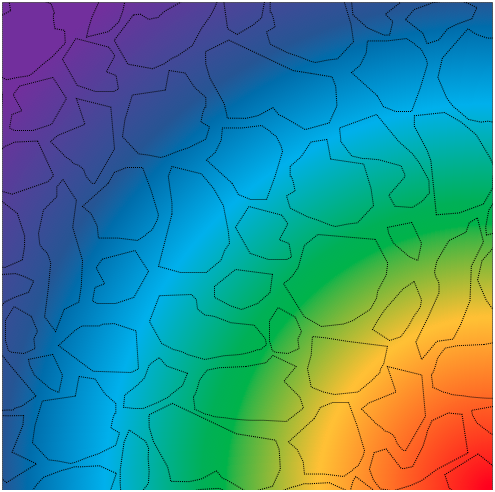
\includegraphics[width=0.8\linewidth]{figs/macro.png}
  \caption{Macroscale \(T_s\) distribution}
  \label{fig:mesoa}
\end{subfigure}
\begin{subfigure}{.485\textwidth}
  \centering
  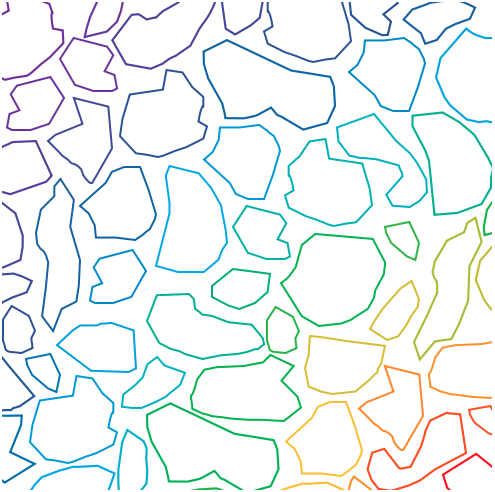
\includegraphics[width=0.8\linewidth]{figs/meso.png}
  \caption{Mesoscale surface BCs}
  \label{fig:mesob}
\end{subfigure}
\caption{Schematic of the (a) macroscale \gls{rev}-averaged solid surface temperature distribution and (b) the uniform surface temperature \gls{bc} on each mesoscale domain.}
\label{fig:meso}
\end{figure}

The spatial distribution of pebbles within the macroscale domain is usually unknown, so the use of the identical pebble representation in Figs. \ref{fig:mesoa} and \ref{fig:mesob} is purely pedagogical. Given the assumption of mesoscale periodicity, the solid surface temperature at each position \(\vec{x}\) in the macroscale domain represents a uniform surface temperature on a representative solid pebble centered at \(\vec{x}\). For the non-spherical pebbles in Fig.\ \ref{fig:mesoa}, each representative pebble may be considered a spherical pebble with a diameter averaged over the actual diameter distribution. 

In solid-fluid mixtures consisting of a homogeneous or multi-layer homogeneous solid phase, the heat equation may readily be applied to estimate the internal solid temperature distribution,

\beq
\label{eq:oem}
\rho_S C_{p,S}\frac{\partial T_S}{\partial t}-\nabla\cdot\left(k_S\nabla T_S\right)-\dot{q}_S=0\ ,
\eeq

\noindent where \(\rho_S\) is the solid density, \(C_{p,S}\) is the solid isobaric specific heat capacity, \(k_S\) is the solid thermal conductivity, \(T_S\) is the internal solid temperature, and \(\dot{q}_S\) is the volumetric heat source. The \(S\) subscript indicates that the thermal properties, volumetric heat source, and temperature correspond to the interior of the solid phase, and is distinct from the \(s\) subscript used to denote the intrinsic phase averaged quantities in the macroscale solid energy conservation equations in Eqs. \eqref{eq:PSEnergy} and \eqref{eq:PSEnergy2}.

To reinforce the conceptual difference between \(s\) and \(S\) subscripts, consider a hypothetical pebble design consisting of three concentric layers of UO$_2$, helium, and zircaloy. Then, \(k_S\) might be specified as

\beq
k_S(r, T_S)=\begin{dcases}
k_{\text{UO}_2}(T_S) & r \leq r_1\\
k_{\text{helium}}(T_S) & r_1 < r \leq r_2\\
k_{\text{zircaloy}}(T_S) & r_2 \leq r < d_p/2\ ,
\end{dcases}
\eeq

\noindent where \(k_{\text{UO}_2}\), \(k_\text{helium}\), and \(k_\text{zircaloy}\) are temperature-dependent thermal conductivity correlations for each layer. The spatial dependence is listed in terms of the radial coordinate due to the uniform surface temperature \gls{bc} and interpretation of each representative pebble as a sphere with average radius \(d_p/2\). \(r_1\) indicates the boundary between the UO$_2$ and helium regions and \(r_2\) indicates the boundary between the helium and zircaloy regions. Similar piecewise expressions would be used for the heat source and the other properties of the solid. Conversely, properties with an \(s\) subscript differ are homogenized over the entire solid phase.

Systems to which this multi-layer homogeneous solid modeling approach is readily applicable include homogeneous graphite pebbles commonly used near outer reflectors in \glspl{pbr} and conventional multi-layer pincell fuels in \glspl{lwr}. \gls{pbr} fuels, on the other hand, are extremely heterogeneous. Fig.\ \ref{fig:pbmr_pebble} shows a pictorial rendering of the fuel pebble design for the \gls{pbmr}, which is representative of many other \gls{pbr} fuels \cite{tecdoc1694}. The pebble consists of two main regions\mdash 1)~a central fuel-matrix region containing approximately 15,000 \glspl{cfp} randomly distributed in a graphite matrix, and 2)~a homogeneous graphite shell protecting the central fuel-matrix region from erosion. The micro length scale characterizes ``representative'' heterogeneous structures within the mesoscale domain; for application to the fuel-matrix region of \gls{pbr} fuels, these heterogeneous structures are the \glspl{cfp}.

\begin{figure}[!h]
\centering
  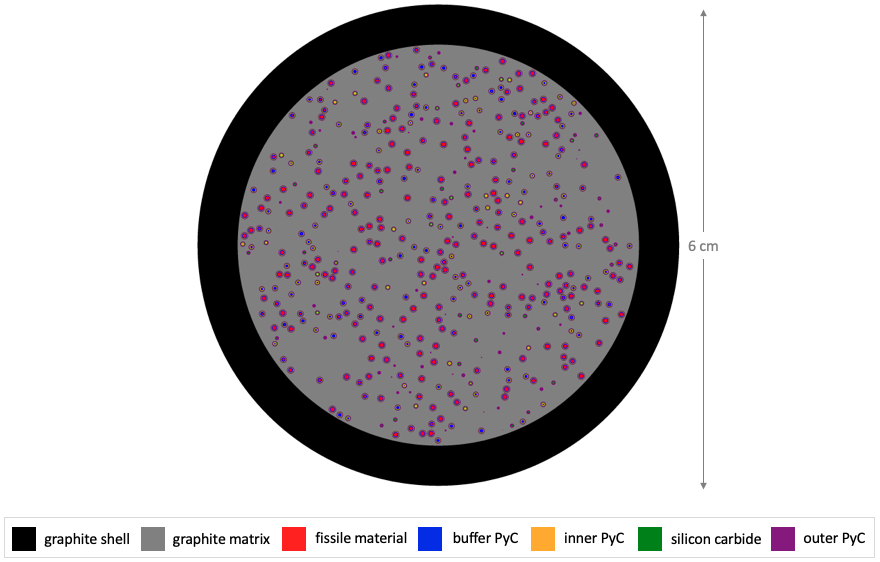
\includegraphics[width=0.85\linewidth]{figs/pbmr_pebble.png}
\caption{Schematic of the \gls{pbmr} fuel pebble design with colors indicating different material compositions.}
\label{fig:pbmr_pebble}
\end{figure}

Many other solid fuel forms encountered in nuclear applications share this heterogeneous character. \gls{fcm} fuels consist of conventional \glspl{cfp} dispersed in a \gls{sic} matrix and fabricated into cylindrical pellets that are intended to replace UO$_2$ pellets in \glspl{lwr} \glspl{htgr} \cite{lu,snead_fcm}. For the conversion of research reactors from high- to low-enriched uranium, either the fuel loading or fissile atom density must be increased to retain the same reactor performance. As the size of the reactors are typically fixed, high fissile density dispersion fuels consisting of U$_3$Si$_2$ or UMo particles in an aluminum matrix have been used \cite{mistarihi,jeong2015}. A fast reactor fuel design consisting of metallic-coated fissile kernels surrounded by a fuel powder matrix has also been proposed \cite{abdalla}.

The different material properties of the \gls{cfp} layers, combined with the localization of the fission heat source to the central \gls{cfp} kernel, necessitates models to describe the microscale structure beyond Eq. \eqref{eq:oem} without explicit representation of all 15,000 particles. Rudimentary models based on volume-averaging the fuel-matrix properties and heat source as inputs to Eq. \eqref{eq:oem} may significantly underpredict fissile kernel temperatures \cite{brown_fcm,kamalpour, novak_2019}.

Multiscale analysis of heterogeneous solids is a large research field, especially in the analysis of conduction through composite materials; as such, a wide variety of methods have been proposed and used. A brief discussion of this research area provides larger context to this work. 

One obvious multiscale model is based on extending the \gls{rev} homogenization of a two-phase fluid-solid domain performed in Section \ref{sec:macro_deriv} to a two-phase soild-solid domain. By interpreting the continuous fluid phase as the solid matrix and the discrete solid pebble phase as the \glspl{cfp}, the spatially homogenized conservation equations in Eq. \eqref{eq:PorousEquations} also apply to the fuel-matrix region of \gls{pbr} fuels. For solid-solid domains, the velocity \(\vec{V}\) is zero such that closure requires specification of the volume fraction of the matrix phase, the effective matrix conductivity, the effective particle conductivity, and the interphase convective heat transfer coefficient. The latter three of these closures can be obtained as extensions of the models described in Sections \ref{sec:Kappa}, \ref{sec:KappaS}, and \ref{sec:alpha}, respectively. The models for \(\kappa_f\) are evaluated with zero thermal dispersion; the models for \(\kappa_s\) are evaluated with the assumption of a transparent solid matrix and no contact conduction component; and the models for \(\alpha\) are evaluated with zero Reynolds number. Other definitions for these closures from Monte Carlo simulations \cite{cho} or mixed diffusion kernels \cite{espinosa} have been proposed. 

A second method, referred to as ``multiscale expansion,'' expresses the temperature as a Taylor series expansion of successive corrections of order \(1\), \(\varsigma\), \(\varsigma^2\), \(\cdots\), where \(\varsigma\) is a small parameter. This ansatz is then plugged into the heat conduction equation and like terms collected to yield a separate differential equation for each correction \cite{weinan}. 

While the spatial homogenization is a natural companion to the macroscale porous media method, its implementation and use is considered as a future research activity. The multiscale expansion method, while mathematically rigorous, results in many unique physics kernels with low reuse potential in a modular computing framework. This method is therefore also not pursued further. The remainder of this section describes two models investigated in this dissertation\mdash the \gls{hl} method and the \gls{hsd} method. Justification for their use over the macroscale homogenization and multiscale expansion methods is provided alongside a technical description.

The \gls{hl} method blends aspects of a multilayer homogeneous solid that can be described by Eq. \eqref{eq:oem} with consideration of the \gls{cfp} layers thermal resistance and heat source localization. The \gls{hl} method is based on symmetrically smearing heterogeneities into a 1-D multilayer solid while preserving volume fractions. Fig.\ \ref{fig:pbmr_hlm} shows one possible representation of the \gls{pbmr} pebble in Fig.\ \ref{fig:pbmr_pebble} with the \gls{hl} method. The total mass of each material is conserved and the geometric structure of the \glspl{cfp} is approximated as a multilayer spherical shell; 15,000 randomly-distributed particles have been simplified to a single pseudo-particle at the expense of a distortion in the thermal resistance seen by the kernel and the separation of a continuous matrix into isolated regions.

\begin{figure}[!h]
\centering
  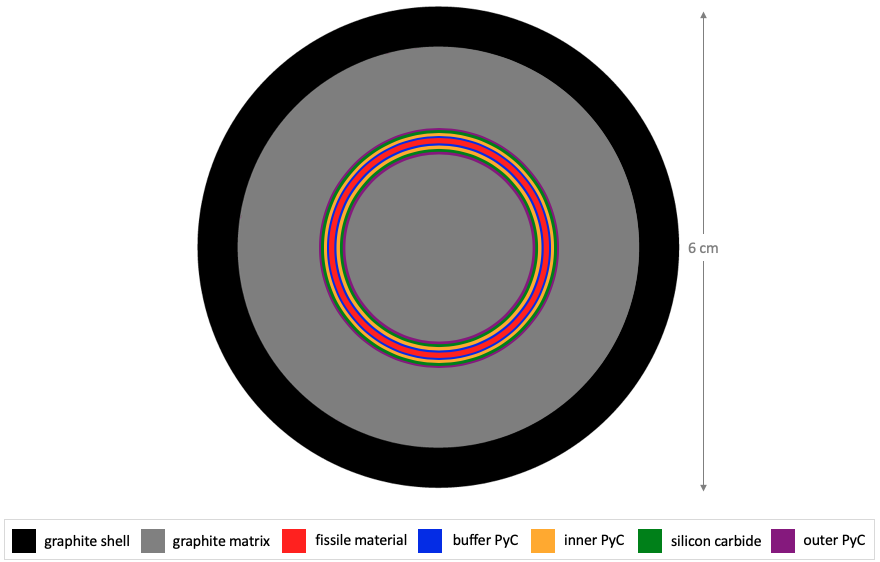
\includegraphics[width=0.85\linewidth]{figs/pbmr_hlm.png}
\caption{Schematic of the \gls{pbmr} fuel pebble design as represented by the \gls{hl} method; colors indicate different material compositions.}
\label{fig:pbmr_hlm}
\end{figure}

Conserving volume fractions of the materials in the fuel-matrix region does not provide a sufficient number of constraints to determine 1)~the number of pseudo-particles; 2)~the location of the pseudo-particles; and 3)~the relative thicknesses of the ``inner'' and ``outer'' layers of non-kernel materials in the pseudo-particles. An infinite number of \gls{hl} representations of the pebble in Fig.\ \ref{fig:pbmr_pebble} can be conceived, so several additional requirements are arbitrarily imposed. 

The number of pseudo-particles \(N_p\) is set as the only free parameter. First, the fuel-matrix region is divided into \(N_p\) equal-volume spherical shells. Consider a shell spanning \(r_i\leq r\leq r_o\) with total volume \(\volume\) given as

\beq
\volume=\frac{4}{3}\pi\left(r_o^3-r_i^3\right)\ .
\eeq

\noindent For a \gls{cfp} packing fraction in the fuel-matrix region of \(\epsilon_\text{cfp}\), \(1-\epsilon_\text{cfp}\) of the shell volume is matrix material. The thickness of the matrix layer along the inner surface, or \(\delta_i\), is chosen such that half of the matrix material is present in a layer along the inner surface. Likewise, the thickness of the matrix layer along the outer surface, or \(\delta_o\), is chosen such that half of the matrix material is present in a layer along the outer surface. In other words, the inner matrix layer thickness is calculated as

\beq
\frac{4}{3}\pi\left\lbrack\left(r_i+\delta_i\right)^3-r_i^3\right\rbrack=\frac{1}{2}\left(1-\epsilon_\text{cfp}\right)\volume\ ,
\eeq

\noindent while the outer matrix layer thickness is calculated as

\beq
\frac{4}{3}\pi\left\lbrack r_o^3-\left(r_o-\delta_o\right)^3\right\rbrack=\frac{1}{2}\left(1-\epsilon_\text{cfp}\right)\volume\ .
\eeq

\noindent A similar process is then performed for the materials in the \gls{cfp}, where the packing fraction of each material in the \gls{cfp} is used to determine the relative volume occupied in the segment.

The \gls{hl} method has no direct correlation to the actual geometry, and temperature solutions should only be used to predict integral metrics such as maximum and average material-wise temperatures. The \gls{hl} method also lacks the mathematical rigor of the approaches described previously. However, the \gls{hl} method is considered here for two reasons \mdash1)~the method is simple to implement and representative of the limitations in single-\gls{pde} fuel models used in many legacy \gls{th} tools; and 2)~the \gls{hl} method has recently been used in preliminary steady-state modeling of \gls{fcm} fuels \cite{brown_fcm} and transient analysis of the Mark-1 \gls{pbfhr} \cite{xin_wang_thesis} that is the subject of the modeling in Chapter \ref{sec:pbfhr}.

The second multiscale model considered is the \gls{hsd} method, which is based on the concept of superposition solutions to linear differential equations \cite{stainsby}. If the heat equation is linear, it may be split into different models for the meso and micro length scales that are superimposed to obtain an approximate temperature solution. A description of the \gls{hsd} method begins by splitting the heterogeneous heat source \(\dot{q}\) into an average \(\la\dot{q}\ra\) and a fluctuation \(\hat{\dot{q}}\),

\beq
\label{eq:heat_source_decomp}
\dot{q}=\la\dot{q}\ra+\hat{\dot{q}}\ ,
\eeq

\noindent where the average of the fluctuation is zero. Each heat source on the \gls{rhs} of Eq. \eqref{eq:heat_source_decomp} is used in a separate conduction equation. The conduction equation based on the average heat source is referred to as the ``mesoscale'' model,

\beq
\label{eq:MesoscaleSolution}
\rho_\text{meso} C_{p,\text{meso}}\frac{\partial T_\text{meso}}{\partial t}-\nabla\cdot(k_\text{meso}\nabla T_\text{meso})-\la\dot{q}\ra=0\ ,
\eeq

\noindent \(\rho_\text{meso}\), \(C_{p,\text{meso}}\), and \(k_\text{meso}\) represent the thermal properties of the heterogeneous domain homogenized in space according to various mixing approaches described in Section \ref{sec:ClosuresMesoMicro}. The mesoscale temperature \(T_\text{meso}\) represents the long-wavelength thermal solution due to the average heat source and average properties. Note that Eq. \eqref{eq:MesoscaleSolution} is very similar to the multi-layer homogeneous solid model in Eq. \eqref{eq:oem}, except that all thermal properties are spatially homogenized and the heat source is averaged over the domain.

The conduction equation based on the fluctuating heat source is referred to as the ``microscale'' model,

\beq
\label{eq:MicroscaleSolution}
\rho_\text{micro} C_{p,\text{micro}}\frac{\partial T_\text{micro}}{\partial t}-\nabla\cdot(k_\text{micro}\nabla T_\text{micro})-\hat{\dot{q}}=0\ ,
\eeq

\noindent \(\rho_\text{micro}\), \(C_{p,\text{micro}}\), and \(k_\text{micro}\) represent the thermal properties resolved on the fine scale; an \(S\) subscript instead of the ``micro'' subscript would also have been appropriate. The microscale temperature \(T_\text{micro}\) represents the small-scale correction to the mesoscale solution.

The approximate temperature solution in the interior solid domain is the superposition of the two solutions,

\beq
\label{eq:MultiscaleSolution}
T_S(\vec{x})=T_\text{meso}(\vec{x})+\sum_{i=1}^{n_p}T_{\text{micro},i}(\vec{x}_i)\ ,
\eeq

\noindent where the summation over the number of \glspl{cfp} \(n_p\) indicates that the microscale solution \(T_{\text{micro},i}\) for the \(i\)-th particle is translated to the location \(\vec{x}_i\) corresponding to the center of that particle. If pebble self-shielding effects are neglected such that the heat source in each particle is identical, a microscale model may be constructed for a single particle and translated to each of the \(n_p\) locations. This simplification is assumed throughout, though it is not an inherent limitation of the method. 

In summary, application of the \gls{hsd} method to the \gls{pbmr} pebble in Fig.\ \ref{fig:pbmr_pebble} involves the following calculation steps\mdash 

\begin{enumerate}
\itemsep0.3em
\item Decompose the heat source into an average and a fluctuation according to Eq. \eqref{eq:heat_source_decomp}.
\item Solve the mesoscale model in Eq. \eqref{eq:MesoscaleSolution} over the entire fuel-matrix region and subject to the \glspl{bc} described in Section \ref{sec:BCsMesoMicro}.
\item Solve the microscale model in Eq. \eqref{eq:MicroscaleSolution} over a single average \gls{cfp} and subject to the \glspl{bc} described in Section \ref{sec:BCsMesoMicro}.
\item Translate the microscale solution to the locations of the 15000 \glspl{cfp} and add to the mesoscale solution according to Eq. \eqref{eq:MultiscaleSolution}.
\end{enumerate}

A verification example that may provide a more intuitive grasp is presented in Section \ref{sec:verification_meso}. The \gls{hsd} method is considered here due to successful application to cylindrical \gls{cfp} compacts that share many similarities to \gls{pbr} fuels \cite{stainsby}.

In practice, the location of each \gls{cfp} is unknown, preventing prediction of the temperature at a specific location. However, often of greater practical interest is the estimation of integral metrics such as maximum and material-wise averaged temperatures. Even if the locations of the heterogeneities are unknown, provided the \glspl{cfp} are randomly dispersed through the domain, the maximum and minimum temperatures in material \(i\) can be approximated as

\beq
\label{eq:MaxT}
\text{max}\left(T_{i}\right)= \text{max}\left(T_\text{meso}\right)+\text{max}\left(T_{\text{micro},i}\right)\ ,
\eeq

\beq
\label{eq:MinT}
\text{min}\left(T_{i}\right)= \text{min}\left(T_\text{meso}\right)+\text{min}\left(T_{\text{micro},i}\right)\ .
\eeq

\noindent In other words, maximum and minimum temperatures are evaluated assuming a microscale domain is situated precisely at the location of the maximum and minimum mesoscale temperatures, respectively. This provides the bounding maximum and minimum temperatures for material \(i\), and hence the actual maximum and minimum temperatures will be within this range given the limitations of the mixing methods used for mesoscale material properties.

In addition, if the mesoscale temperature solution varies over a longer length scale than the size of the \glspl{cfp}, the average temperature in material \(i\) can be approximated as

\beq
\label{eq:AvgT}
\la T_i\ra=\la T_\text{meso}\ra+\la T_{\text{micro},i}\ra\ .
\eeq

\noindent Note that while Eq. \eqref{eq:ConstantShiftMMD} requires the average of the microscale solution over the entire microscale domain to be zero, the $i$ subscript in Eq. \eqref{eq:AvgT} represents the average over only the $i$-th material layer in the microscale domain. The approximation in Eq. \eqref{eq:AvgT} is frequently applicable to \gls{pbr} fuels because the micro length scale is approximately 50 times smaller than the meso length scale, and extremely different particle-to-particle powers or non-uniform matrix-shell \glspl{bc} are uncommon.

The most important assumption made in the \gls{hsd} method is that the heat equation is linear, and thus amenable to superposition techniques. Linearity implies that the thermal properties are independent of temperature. In this dissertation, the mesoscale and microscale models are applied to steady-state analysis of the Mark-1 \gls{pbfhr}. The \gls{pbfhr} core temperature rise of 100\si{\celsius}, the close proximity of the \glspl{cfp} to the pebble surface, and the distribution of the pebble power among a relatively high number of \glspl{cfp} per pebble result in pebble temperature distributions that vary relatively little throughout the bed as compared to other nuclear fuels such as \gls{uo2} fuels in \glspl{lwr} and \glspl{sfr}. 

Based on the solid properties provided in Appendix \ref{sec:props}, a \(\pm\)100\si{\celsius} change in temperature relative to 1000\si{\kelvin} results in approximately a \(\mp\)5\%, \(\mp\)10\%, and \(\mp\)10\% change in the matrix graphite, \gls{uo2}, and \gls{sic} thermal conductivities, respectively. To the author's knowledge, temperature-dependent models are unavailable for porous and pyrolitic graphite. These relatively small variations with temperature justify the use of thermal properties evaluated at the bed-averaged temperature.

Transient modeling, especially in scenarios with large power changes such as \glspl{ria}, must consider temperature dependence. There are a number of ways in which some property temperature dependence can be retained. The \gls{hsd} method can be applied iteratively in a number of discrete heterogeneous regions, each with unique thermal properties evaluated at the average temperature of the region. Or, unique thermal properties may be used for each pebble according to its location in the macroscale solid temperature field. Future work will incorporate temperature dependence in the \gls{hsd} method.

In most \glspl{pbr}, of equal or greater concern is the dependence of thermal properties on burnup. This dependence can be easily accommodated provided the burnup over a pebble is assumed uniform by using constant thermal properties evaluated at a particular burnup level.

\subsection{Boundary and Initial Conditions}
\label{sec:BCsMesoMicro}

Most \gls{pbr} fuels contain a surface layer of homogeneous graphite to protect the fuel-matrix region from erosion. The surface temperature of a representative pebble in each computational element is taken as the average macroscale solid surface temperature over the element, or \(T_{s,\text{avg}}\). The \gls{hl} method is applied over both the heterogeneous fuel-matrix region and the homogeneous graphite shell, so a temperature \gls{bc} on the pebble surface \(\Gamma_p\) is specified as

\beq
\label{eq:PebSurf}
T_S\rvert_{\Gamma_p}=T_{s,\text{avg}}\ .
\eeq

\noindent The \gls{hsd} method involves coupled solutions on two length scales and summing those solutions together as in Eq. \eqref{eq:MultiscaleSolution}. Unlike the \gls{hl} method, the \gls{hsd} method is only applied in heterogeneous regions. In the homogeneous graphite shell, the temperature distribution is obtained by solution of Eq. \eqref{eq:oem} with surface \gls{bc} given by Eq. \eqref{eq:PebSurf}. At the interface between the homogeneous shell and the fuel-matrix region, continuity of temperature and heat flux with the homogeneous shell is required.

\begin{comment}
\beq
\label{eq:MesoShift}
\left(T_\text{meso}+T_\text{micro}\right)\rvert_{\Gamma_i}=T_S\rvert_{\Gamma_i}\ ,
\eeq

\beq
\label{eq:MesoShift2}
\left(-k_\text{meso}\nabla T_\text{meso}\cdot\hat{n}-k_\text{micro}\nabla T_\text{micro}\cdot\hat{n}\right)\rvert_{\Gamma_i}=-k_S\nabla T_S\cdot\hat{n}\rvert_{\Gamma_i}\ .
\eeq
\end{comment}

In addition, the microscale solution must have a zero average over the microscale domain in order to represent a zero-average fluctuation on the long-wavelength mesoscale solution. This is enforced by applying a Dirichlet \gls{bc} on the boundary \(\Gamma_\text{micro}\) of the microscale domain such that the average of the microscale solution over the microscale volume \(\volume_\text{micro}\) is zero,

\beq
\label{eq:ConstantShiftMMD}
T_\text{micro}\rvert_{\Gamma_m} =-\frac{1}{\volume_\text{micro}}\int_{\volume_\text{micro}} T_\text{micro}d\volume\ .
\eeq

\subsection{Closures}
\label{sec:ClosuresMesoMicro}

This section describes models used for the mesoscale and microscale closures. Section \ref{sec:micro_props} describes models for the locally resolved properties \(\rho_\text{micro}\), \(C_{p,\text{micro}}\), and \(k_\text{micro}\), while Section \ref{sec:meso_props} describes models for the spatially homogenized mesoscale properties \(\rho_\text{meso}\), \(C_{p,\text{meso}}\), and \(k_\text{meso}\).


\subsubsection{Microscale Solid Properties}
\label{sec:micro_props}

Both the \gls{hl} and \gls{hsd} methods require the internal solid properties \(\rho_S\), \(C_{p,S}\), and \(k_S\) for closure; in the context of the \gls{hsd} method, these properties have been represented equivalently with the notation \(\rho_\text{micro}\), \(C_{p,\text{micro}}\), and \(k_\text{micro}\). Correlations for density, isobaric specific heat, and thermal conductivity of pure, un-mixed, solid materials as a function of internal solid temperature is provided in Appendix \ref{sec:props}.

\subsubsection{Mesoscale Solid Properties}
\label{sec:meso_props}

The spatially homogenized properties \(\rho_\text{meso}\), \(C_{p,\text{meso}}\), and \(k_\text{meso}\) represent effective properties of a heterogeneous solid. The homogenization models described in this section assume that these effective properties are a combination of the properties of its constituents.

%It is also assumed that all of the materials to be mixed are at the same temperature.

Consider a mixture of materials \(i\) for \(i=1\ ...\ N_m\) each with a phase fraction \(\epsilon_i\) and generic property \(\chi_i\). These phase fractions sum to unity. The simplest method for determining average properties is the use of series combination,

\beq
\label{eq:series}
\chi=\sum_{i\ =\ 1}^{N_m}\epsilon_i\chi_i\ ,
\eeq

\noindent which is equivalent to a volume average. Alternatively, a parallel combination may be used,

\beq
\label{eq:parallel}
\frac{1}{\chi}=\sum_{i\ =\ 1}^{N_m}\frac{\epsilon_i}{\chi_i}\ .
\eeq

\noindent Specifically for binary systems such as the particle-matrix system, many theoretical models based on the notion of transport have been developed. Chiew and Glandt extended Maxwell's potential theory for randomly-distributed, non-interacting, spheres \cite{progelhof} to higher order, giving

\beq
\label{eq:ChiewGlandt}
\chi=\chi_c\frac{1+2\beta_n\epsilon_d+\left(2\beta_n^3-0.1\beta_n\right)\epsilon_d^2+0.05\epsilon_d^3\exp{(4.5\beta_n)}}{1-\beta_n\epsilon_d}\ ,
\eeq

\noindent where \(\beta_n\) is defined as

\beq
\label{eq:betanDef}
\beta_n\equiv\frac{\chi_d-\chi_c}{\chi_d+2\chi_c}\ ,
\eeq

\noindent and \(c\) subscripts indicate the continuous phase and \(d\) subscripts indicate the dispersed phase \cite{kamalpour,liu,gonzo,folsom}. Lewis and Nielsen developed a similar extension to Maxwell's theory as \cite{nielsen,progelhof}

\beq
\label{eq:Nielsen}
\chi=\chi_c\frac{1+1.5\beta_m\epsilon_d}{1-\beta_m\epsilon_d\left(1+\frac{1-0.637}{0.637^2}\ \epsilon_d\right)}\ ,
\eeq

\noindent where \(\beta_m\) is defined as

\beq
\label{eq:BmDef}
\beta_m\equiv\frac{\chi_d-\chi_c}{\chi_d+1.5\chi_c}\ .
\eeq

\noindent For solids with multiple layers of heterogeneity, such as most \gls{pbr} fuels, properties are first homogenized beginning on the fine scales and then on increasingly coarse scales. In this work, either Eq. \eqref{eq:ChiewGlandt} or Eq. \eqref{eq:Nielsen} is used for averaging the fuel matrix with the \glspl{cfp}, while either Eq. \eqref{eq:series} or Eq. \eqref{eq:parallel} are used for all other averages. 

Take the \gls{pbmr} pebble in Fig.\ \ref{fig:pbmr_pebble} as an example, with Eq. \eqref{eq:series} used for all averages except the \glspl{cfp} with the matrix. The intrinsic phase average of a property \(\chi\) over the pebble is calculated as

\beq
\label{eq:NonTransport2}
\chi_s= \epsilon_\text{fm}\chi_\text{fm}+(1-\epsilon_\text{fm})\chi_{gs}\ ,
\eeq

\noindent where \(\epsilon_\text{fm}\) is the volume fraction of the pebble that is the fuel-matrix region, \(\chi_\text{fm}\) is the average of \(\chi\) over the fuel-matrix region, and \(\chi_{gs}\) is the property of the graphite shell. \(\chi_\text{fm}\) is calculated as

\beq
\label{eq:NonTransport}
\chi_\text{fm}= \epsilon_\text{cfp}\chi_\text{cfp}+(1-\epsilon_\text{cfp})\chi_\text{mat}\ ,
\eeq

\noindent where \(\epsilon_\text{cfp}\) is the volume fraction of the fuel-matrix region that is \glspl{cfp}; \(\chi_\text{cfp}\) is the average of \(\chi\) over a \gls{cfp} using the series average in Eq. \eqref{eq:series}; and \(\chi_\text{mat}\) is the property of the matrix. 

For \gls{pbr} applications, the mesoscale properties indicated generically by \(\rho_\text{meso}\), \(C_{p,\text{meso}}\) and \(k_\text{meso}\) are equivalent to \(\rho_\text{fm}\), \(C_{p,fm}\) and \(k_\text{fm}\). The intrinsic solid phase averaged properties \(\rho_s\), \(C_{p,s}\), and \(k_s\) required in the macroscale model are computed using these homogenization models over the entire pebble.

\section{Limitations, Assumptions, and Knowledge Gaps}
\label{sec:MacroAssumptions}

Many assumptions were made explicitly or implicitly in the derivation of the macroscale spatially homogenized conservation equations in Section \ref{sec:macro_deriv} and in the models selected for the meso and micro length scales in Section \ref{sec:mesomicro}. Assumptions have been made in 1)~the form of the local conservation equations in Eqs. \eqref{eq:ContinuityNonPorous}--\eqref{eq:EnergyNonPorous}, and \eqref{eq:InternalEnergy}, 2)~in the spatial homogenization procedure used to obtain the macroscale model in Eqs. \eqref{eq:PorousEquations} and \eqref{eq:PrimitiveEqns}, and 3)~in the implementation details of the \gls{hl} and \gls{hsd} methods. Existing closure models applicable to \glspl{pbr} also exhibit many limitations and knowledge gaps at all three length scales. A brief summary is now provided of the limitations, assumptions, and knowledge gaps that have the largest impact on the general applicability of this multiscale method to modeling of \glspl{pbr}.

Both the local mass conservation in Eq. \eqref{eq:ContinuityNonPorous} and the two-phase homogenization assume a single phase fluid and no mass transfer between the fluid and solid phases. The macroscale model therefore cannot model multi-phase fluid flow, such as water ingress events important to safety analysis of \glspl{htgr}. The assumption of a pure, simple, fluid in the conservation of energy equations excludes analysis of reacting flows. The macroscale \glspl{bc} assume the flow is subsonic. 

There are several inherent limitations of the macroscale modeling approach with regards to predicting key safety metrics such as maximum fuel temperature. Because porous media models are based on spatial averaging, all local flow and heat transfer effects are only retained in an average sense. The distribution of temperature on an individual pebble surface or reflector block is unknown. Resolved \gls{cfd} simulations of pebbles show that surface temperatures are tens to hundreds of degrees higher, depending on the flow conditions, at stagnation points and near the low-flow recirculation regions behind pebbles than near thin, main-flow aligned, gaps \cite{bai,ferng,ge,lee2007,song,wu2010}. This surface temperature distribution affects the maximum fuel temperature, but the macroscale model is restricted to predicting the mesoscale and microscale temperatures based on a surface-uniform solid temperature, and hence will underpredict the true maximum fuel temperature. \gls{cfd} simulations of fluid flow around pebbles with the \glspl{cfp} resolved within each pebble are required to estimate the extent to which a uniform pebble surface temperature underpredicts the true maximum fuel temperature. The large temperature margins to \gls{cfp} failure often permit the use of safety factors to conservatively account for this effect. However, reactors with higher power densities and operating temperatures may have smaller margins to failure and require more refined analysis.

Chemical reactions are frequently strong functions of temperature. In addition to underpredicting the true maximum fuel temperature, the homogenization of the pebble surface temperature will underpredict the variation in chemical reaction rates over the surface of a pebble. For example, Fig.\ \ref{fig:corroded_pebble} shows a graphite pebble, originally spherical in shape, with significant and nonuniform oxidation that may have been caused by nonuniform surface temperature distributions. Similar stagnation-related chemical reactions have resulted in coolant polymerization in organic-cooled reactors \cite{shirvan}. Extensive dimensional changes may result in further amplification of surface temperature non-uniformity and complicate pebble handling systems. 

Spatial homogenization may also fail to correctly capture mass transfer processes such as tritium uptake in the pebbles of lithium-bearing salt-cooled systems. Further investigation is needed to better understand the effect of spatial homogenization on prediction of integral chemical reaction and mass transfer rates.

% Stagnation points usually occur at or near the pebble contact points that are not aligned with the flow direction due to vortex formation and back flow \cite{lee_lee, hassan, ge,king}. Nusselt numbers typically range between 10 and 150 over the surface of a single pebble \cite{ferng}.

\begin{figure}[!h]
\centering
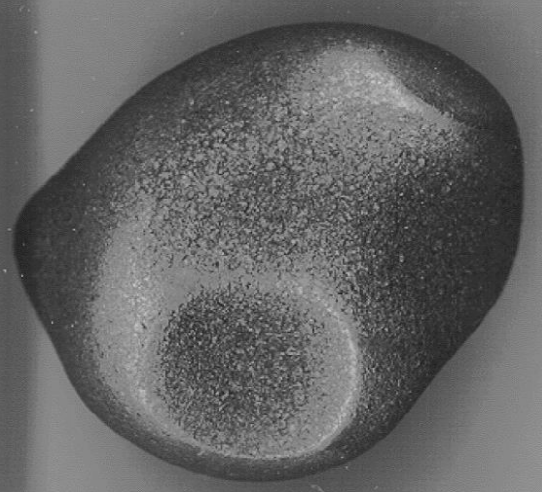
\includegraphics[width=0.4\linewidth]{figs/corroded_pebble.png}
\caption{Corroded graphite pebble, originally spherical in shape, with nonuniform oxidation damage from the KFA Veluna experiment \cite{hassan_mev}.}
\label{fig:corroded_pebble}
\end{figure}

%Provided the neutron migration length is larger than the porous media averaging length, the use of a porous media \gls{th} solution for temperature feedback in neutronics simulations is an acceptable simplification of the fluid flow and heat transfer \cite{aufiero_2016, rintala}.

In addition to the assumptions and limitations inherent in the macroscale model, the existing literature on macroscale closures is characterized by many knowledge gaps that affect the applicability of this form of multiscale analysis to \glspl{pbr}. The remainder of this section highlights several of these gaps in order to motivate future experimental programs aimed at closure refinement. Most of the emphasis is placed on the interphase friction factor \(W\), interphase convective heat transfer coefficient \(\alpha\), and effective solid thermal conductivity \(\kappa_s\), rather than on the porosity \(\epsilon\), Brinkman viscosity \(\tilde{\mu}\), and effective fluid thermal conductivity \(\kappa_f\). This emphasis is justified because the field of \gls{dem} modeling is well-established and equipped with methods for predicting porosity in complex domains, provided accurate data is available for pebble material properties such as roughness and elastic modulus \cite{lammps,openfoam,liggghts,zhang2001}. However, the assumption of a time-independent porosity precludes analysis of large-motion events such as earthquakes, and future work may incorporate \gls{dem} modeling to obtain more accurate predictions of porosity. Further, the Brinkman viscosity and effective fluid thermal conductivity are seldom used in modeling of \glspl{pbr}, and flow and temperature predictions are relatively insensitive to their selection \cite{auwerda_2011,tecdoc1163}.

Generally speaking, models for \(W\), \(\alpha\), and \(\kappa_s\) are based on experimental data measured at the inlet and outlet of a bed. For example, a model for \(W\) would be developed by fitting pressure drop data obtained as differences between the inlet and outlet pressure along the centerline of a pipe containing a packed bed. The most significant knowledge gap for macroscale closures is the lack of a spatial dependence that explicitly considers the very different \gls{th} effects in the near-wall versus bulk regions of the bed. The porosity that appears in these closure models represents the bed-averaged porosity. A common, but crude, approximation attempts to extend bulk bed correlations to the near-wall regions by interpreting the porosity as the local porosity \cite{kaviany, vortmeyer, giese, vafai}. However, many of the macroscale closures predict unphysical behavior as porosity tends to unity. For example, the hydraulic diameter in Eq. \eqref{eq:Dh} and \(\kappa_\text{radiation}\) in Eq. \eqref{eq:KappaRadiationBB} both tend to infinity.

As discussed in greater detail in Chapter \ref{sec:sana}, the lack of models correlated for the near-wall region may contribute to significantly higher errors in temperature predictions in these regions \cite{novak_2019}. Experimental and numerical investigations are required to develop macroscale closures applicable to the near-wall region, as well as supporting parameters such as the hydraulic diameter. The \gls{neams} funding call in 2019 titled ``Near-Wall Gas-Flow Correlations in Pebble Bed Reactors'' points to the importance of addressing this knowledge gap for \gls{pbr} thermal analysis \cite{neams2}. 

Even in the bulk region, a number of important assumptions have been made. The model for \(\kappa_\text{radiation}\) in Eq. \eqref{eq:KappaRadiationBB} applies to a transparent fluid. While many pure salts are broadly transparent, absorption coefficients may be five times higher upon the addition of impurities such as chromium \cite{chaleff}. In addition, few macroscale closure models consider any entrance length effects, and inconsistencies are commonly observed in proposed modifications for entrance regions. For example, the Nusselt number is generally larger in the first few sphere layers because of thinner boundary layers \cite{ferng,song}. However, others have observed the opposite \cite{KTAhtc} or no effect \cite{song}, which may be attributable to differences in packing structure and the counteracting effect of absent turbulent wakes from upstream pebbles \cite{achenbach}. 

At the meso and micro length scales, the heterogeneous pebble geometry has been dramatically simplified through either the \gls{hl} or \gls{hsd} method. In this dissertation, the effect of self-shielding on \gls{cfp} power distribution has been neglected, and thermal properties in the \gls{hsd} are assumed independent of temperature. 

Finally, all three length scales are affected by uncertainties in fundamental fluid and solid properties, as well as in their effective mixed state. The strong dose dependence on graphite properties is neglected \cite{seker}, and the dependence of \gls{cfp} layer properties on manufacturing conditions is not considered. In the mixing of component properties to estimate effective properties, it is assumed that the properties of an individual component in a mixture are the same as the properties of the corresponding pure material. This simplification neglects differences in microstructure between the pure components and the mixture, which can be significant in graphite and \gls{fcm} fuels \cite{folsom,lee2017}.


% TODO: literature review of CFD of pebble beds
\begin{comment}


Most experiments and simulations show a higher pressure drop per unit length in the first several sphere layers than in the bulk \cite{baker_2010}, though others have not observed any entrance region effect \cite{calis,bai_2009,zhang2016}. 

These different reported entrance effects for Nusselt number and friction factor remain to be reconciled as functions of packing and flow regime.

%\cite{bai} fits drag with polynomial in Re, gives bad results at high Re
\end{comment}

% uncertainties in the correlations
%Maximum temperatures are in some cases very sensitive to the models used for \(\kappa_s\) \cite{sana_report,becker}. Contributing to this sensitivity are the relatively high uncertainties reported in many experimental measurements, which may be partially attributable to the sensitivity of contact conduction to corrosion \cite{aichlmayr}, the sensitivity of the thermal conductivity to the oxidation state \cite{swift}, and/or the presence of small convection currents \cite{nozad}.

